\documentclass{sig-alternate}

\usepackage{xspace,xcolor}
\usepackage{graphicx,hyperref,color}
\usepackage{algorithm,algorithmic}

\begin{document}
\conferenceinfo{SOCC'12,} {October 14-17, 2012, San Jose, CA USA} 
\CopyrightYear{2012}
\crdata{978-1-4503-1761-0/12/10}
\clubpenalty=10000
\widowpenalty = 10000 

\newcommand{\eat}[1]{}
\newcommand{\eg}{{\em e.g.}, }
\newcommand{\ie}{{\em i.e.}, }
\newcommand{\etc}{{etc.}\xspace}
\newcommand{\etal}{{\em et al.\ }}

\newcommand{\subheader}[1]{\noindent \textbf{#1}}

\newcommand{\linkedin}{{LinkedIn}\xspace}
\newcommand{\helix}{{Helix}\xspace}
\newcommand{\ES}{{Espresso}\xspace}
\newcommand{\databus}{{Databus}\xspace}
\newcommand{\GP}{{Galapagos}\xspace}
\newcommand{\sensei}{{Sensei}\xspace}
\newcommand{\seas}{{Search-as-a-service}\xspace}
\newcommand{\mysql}{{MySQL}\xspace}

\title{Untangling Cluster Management with \helix}

\def\sharedaffiliation{%
\end{tabular}
\begin{tabular}{c}}

\numberofauthors{1}
\author{
\alignauthor Kishore Gopalakrishna, Shi Lu, Zhen Zhang, Adam Silberstein,\\ 
 Kapil Surlaker,Ramesh Subramonian, Bob Schulman \\
%
\sharedaffiliation
\affaddr{LinkedIn}\\
\affaddr{Mountain View, CA, USA}\\
\affaddr{\{kgopalakrishna,slu,zzhang,asilberstein,ksurlaker,rsubramonian,bob\}@linkedin.com}
}

\newcommand{\aes}[1]{\textcolor{green}{\bf AES: #1}}
\newcommand{\TBC}{{\framebox{\textbf{TO BE COMPLETED }}}}
\newcommand{\TBCKS}{{\framebox{\textbf{TO BE COMPLETED KAPIL}}}}
\newcommand{\TBCKG}{{\framebox{\textbf{TO BE COMPLETED KISHORE}}}}
\newcommand{\TBCSG}{{\framebox{\textbf{TO BE COMPLETED RAMESH}}}}


\newcommand{\bi}{\begin{itemize}}
\newcommand{\ei}{\end{itemize}}
\newcommand{\bd}{\begin{description}}
\newcommand{\ed}{\end{description}}
\newcommand{\be}{\begin{enumerate}}
\newcommand{\ee}{\end{enumerate}}

\newcommand{\squishlist}{
   \begin{list}{$\bullet$}
    {
      \setlength{\itemsep}{0pt}
      \setlength{\parsep}{3pt}
      \setlength{\topsep}{3pt}
      \setlength{\partopsep}{0pt}
      \setlength{\leftmargin}{1.5em}
      \setlength{\labelwidth}{1em}
      \setlength{\labelsep}{0.5em} } }

\newcommand{\squishlisttwo}{
   \begin{list}{$\bullet$}
    {
      \setlength{\itemsep}{0pt}
      \setlength{\parsep}{0pt}
      \setlength{\topsep}{0pt}
      \setlength{\partopsep}{0pt}
      \setlength{\leftmargin}{2em}
      \setlength{\labelwidth}{1.5em}
      \setlength{\labelsep}{0.5em} } }


\newcommand{\squishend}{
    \end{list}  }

\newtheorem{definition}{Definition}
\newtheorem{theorem}{Theorem}
\newtheorem{lemma}{Lemma}
\newtheorem{claim}{Claim}
\newtheorem{notation}{Notation}
\newtheorem{invariant}{Invariant}
\newcommand{\ccc}{sample command}

\maketitle

Distributed data systems systems are used in a variety of
settings like online serving, offline analytics, data 
transport, and search, among other use cases.  They let organizations scale out their 
workloads using cost-effective commodity hardware, while retaining key properties 
like fault tolerance and scalability.  At \linkedin we have built a number of
such systems.  A key pattern we observe is that even though they may serve different purposes, 
they tend to have a lot of common functionality, and tend to use common building blocks 
in their architectures.  One such building block that is just beginning to
receive attention is cluster management, which addresses 
the complexity of handling a dynamic, large-scale system with many servers.  
Such systems must handle software and hardware failures, 
setup tasks such as bootstrapping data, and
operational issues such as data placement, load balancing, planned upgrades, and cluster expansion.  
 
All of this shared complexity, which we see in all of our systems, motivates us
to build a cluster management framework, \helix, to solve these problems once in a
general way.

\helix provides an abstraction for a system developer to separate coordination and management tasks
from component functional tasks of a distributed system.  The developer defines the system behavior via a 
state model that enumerates the possible states of each component, the transitions between those states, 
and constraints that govern the system�s valid settings. \helix does the heavy lifting of
ensuring the system satisfies that state model in the distributed setting,
while also meeting the system's goals on load balancing and throttling state
changes.
We detail several \helix-managed production distributed systems 
at \linkedin and how \helix has helped them avoid building custom management components.  
We describe the \helix design and implementation and present an experimental
study that demonstrates its performance and functionality.



\vspace{2mm}

\noindent
{\bf Categories and Subject Descriptors:} H.3.4 {[Systems and
    Software]}: {Distributed systems}

\noindent
{\bf General Terms:} Design, Algorithms


\section{Introduction}
\label{sec:intro}
%
The number and variety of distributed data systems (DDSs) have grown
dramatically in recent years and are key infrastructure pieces in a variety of
industrial and academic settings.    
These systems cover a number of use cases including online serving,
offline analytics, search, and messaging.  The 
appeal of such systems is clear: they let developers solve large-scale data 
management problems by letting them focus on business logic, rather than hard distributed systems problems
like fault tolerance, scalability, elasticity, \etc   And because these systems
deploy on commodity hardware, they let organizations avoid purchasing and
maintaining specialized hardware. 
 
At \linkedin, as at other web companies, our infrastructure stack follows the
above model~\cite{linkedin12}.  Our stack includes offline data storage, data
transport systems \databus and Kafka, front end data serving systems Voldemort
and \ES, and front end search systems.  We see the same model repeated in a
variety of other well-known systems like
Hadoop~\cite{hadoop}, HBase~\cite{hbase}, Cassandra~\cite{cassandra},
MongoDB~\cite{mongodb} and Hedwig~\cite{hedwig}.  
These systems serve a variety of purposes and each provides unique features and tradeoffs, yet 
they share a lot of functionality.  As evidence of shared functionality, we
observe systems frequently reusing the same off-the-shelf components.  A primary
example is at the storage layer of DDSs.
PNUTS~\cite{cooper08}, Espresso~\cite{linkedin12}, and others use \mysql 
as an underlying storage engine, different Google systems build on
GFS~\cite{chang06, shute12}, and HBase~\cite{hbase} builds on HDFS.  These storage
engines are robust building blocks used here for lowest-level storage, while
other key features like partitioning, replication, \etc are built at higher layers.  

The storage layer, however, is by no means the only component amenable to
sharing.  What has been missing from \linkedin's and other DDS stacks is shared
cluster management, or an operating system for the 
\\ cloud~\cite{zaharia11}.
DDSs have a number of moving parts, often carrying state.  Much of a system�s complexity is devoted 
toward ensuring these components are all alive and running effectively, bootstrapping new components
to replace failed ones, etc.  Handling failures, planned upgrades, background tasks such as backups,
coalescing of data, updates, rollbacks, cluster expansion, and load balancing all require coordination
that cannot be accomplished easily or effectively within the components themselves. 
Coordination is a first-class function of a DDS.  By separating it into a cluster management component, 
the functional components of the distributed system are simpler to build.  

\subheader{Cluster Management}
The term \emph{cluster management} is a broad one.  We define it as the set of
common tasks required to run and maintain a DDS.  These tasks are:
\squishlist
\item \emph{Resource management}: The resource (database, index, \etc) the DDS
provides must be divided among different nodes in the cluster.
\item \emph{Fault tolerance}: The DDS must continue to function amid node
failures, including not losing data and maintaining read and write availability.
\item \emph{Elasticity}: As workloads grow, clusters must grow to meet increased
demand by adding more nodes.  The DDS's resources must be
redistributed appropriately across the new nodes.
\item \emph{Monitoring}: The cluster must be monitored, both for component
failures that affect fault tolerance, and for various health metrics such as load 
imbalance and SLA misses that affect performance.  Monitoring requires followup
action, such as re-replicating lost data or re-balancing data across nodes. 
\squishend
\eat{%%%%%%%
\squishlist
\item \emph{Bootstrapping}: Systems startup with a careful set of choreographed steps.  For example, 
a server may be assigned a set of data partitions and then create empty data
stores for the partitions, optionally load the partitions from backups, and then
make each partition available for serving.  The
server must progress through these steps sequentially and retry when any fail.
\item \emph{Deployment constraints}: Systems typically constrain how data is
distributed across it.  For example, a systems may enforce a minimum number of
replicas per data partition, and that no replicas of the same partition can be
co-located on a server. 
\item \emph{Failure detection and health monitoring}: Systems must have
monitoring for component failures, as well as various health metrics, 
such as latency SLA misses or load imbalance.
\item \emph{Rebalancing for failures/load/elastic expansion}: Systems must
respond to changes in load and changes to the cluster.   Some examples are the
ability to respond to failures (\eg by re-replicating under-replicated partitions) and to performance 
degradation (\eg by shifting partitions from heavily-loaded servers to lightly-loaded servers).  
Over time we may need to add more capacity to a system, and then must similarly shift load to new servers.
\squishend
}%%%%%%%%%%
We more formally define DDS cluster management tasks in
Section~\ref{sec:requirements}. 


Despite so much common ground, there is not a large and mature body of work in making cluster management a
 standalone generic building block as compared to the storage layer. 
That said, there is a burgeoning body of work in this area
(as seen in YARN~\cite{yarn} and other systems discussed in
Section~\ref{sec:related}).  

There are a number of possible reasons.  In the evolution of a DDS, the
storage layer provides the primary functionality, and the capabilities required to 
manage and operate the cluster become apparent incrementally as the system is deployed. 
The most expedient way to add those capabilities is to incorporate them into the DDS components.
It is not obvious in the early stages that generic cluster management functionality will be required, 
and as those capabilities are added, the system becomes more complex.  We have found that it is possible 
to separate the cluster management tasks, and build multiple systems using a generic, standalone cluster
 manager 
    
While defining and building a generic cluster management system is a daunting
challenge, the benefits are immense for a company like \linkedin.  We are
building out many DDSs.  If each of these can rely on a single cluster manager,
we gain a lot of benefit from simpler and faster development time, as well as
operational simplicity.  

\textbf{\helix} This paper presents \helix, a generic cluster management system we have developed at LinkedIn.  
\helix Helix drastically simplifies cluster management by providing a simple abstraction for describing DDSs and 
exposing to DDS a set of pluggable interfaces for declaring their correct behavior.

\eat{%%%%%%
Briefly, a DDS runs on a cluster consisting of
multiple nodes (\ie servers).  The DDS manages one or more resources, such as a
database or index; since resources can be very large, they are divided into one
or more partitions.  We fully distill a DDS's components in
Section~\ref{sec:requirements}.
}%%%%%%%%

Key among the pluggable interfaces is
an augmented finite state machine, which the DDS uses
to encode its valid settings, \ie its possible states and
transitions, and associated constraints.   The 
DDS may also specify, using an optimization module, goals for how its resources are best distributed over a cluster, \ie
how to place resources and how to throttle cluster transitions.  
\helix uses these to guide the actions it executes on the various
components of the DDS.  This includes monitoring 
system state for correctness and performance, and executing system transitions as
needed.  \helix automatically ensures the DDS is always valid, both in steady state and while
executing transitions, and chooses optimal strategies during state changes, given the defined constraints. 
This approach lets DDS
designers focus on modeling system behavior, rather than the complexity of choreographing 
that behavior.

In this paper we make the following contributions:
\squishlist
\item A model for generic cluster management, including both defining the common
components of a DDS and the functionality a cluster manager must provide (Section~\ref{sec:requirements}).
\item The design and implementation of \helix.  This includes its pluggable
interfaces and examples of how we use
it at \linkedin to support a diverse set of production systems. 
We initially targeted a diverse set of systems: \ES, a serving store; \databus, a change capture and 
transport system, and a \seas system.  (Sections~\ref{sec:design} and \ref{sec:arch}).
\item An experimental study of \helix.  We show that \helix is highly responsive to
key events like server failure.  We also show how through generic cluster
management we make it possible to debug DDS correctness while remaining
agnostic to the DDS's actual purpose. (Section~\ref{sec:eval}).  
\squishend
We review related work in Section~\ref{sec:related}.  We conclude and handle
future work in Section~\ref{sec:conclusion}.

\section{Motivation}
\label{sec:motivation}
%
At \linkedin we have built and deployed a number of DDSs.
These DDSs have many common characteristics in how
they are deployed, monitored, expanded, \etc and differences in specific optimization goals,
constraints, \etc on how those commonalities must happen.
The goal of building a general cluster manager is very appealing for \linkedin and the community.  
Providing a common way for a system to declare 
its own model, without worrying about how to force the system to conform to that model, makes creating 
that model easy and uniform.  Moreover, it simplifies operational support, since there is only one 
cluster manager executing cluster changes across different systems, and we can concentrate on that 
manager's correctness.

  Our goal in this work is to 
formally identify the common characteristics of DDSs and then build a cluster manager that 
both handles those requirements for the DDS, while exposing interfaces so the DDS can declaratively
describe their own system-specific model of behavior.  The cluster manager
itself does the heavy lifting on the DDS. 

 

\subsection{Use Cases}
\label{sec:usecases}
%
Before delving into cluster manager requirements, it helps to review a sample of DDSs that we 
target.  We describe three \linkedin systems.  We have purposefully chosen them for their diversity,
to ensure the commonalities we draw from them are truly found in most or all DDSs.  These use cases
are good as examples, but are also the some of the earliest use cases at \linkedin that motivated our 
cluster management work.

\subheader{Espresso}
Espresso is a distributed, timeline consistent, scalable, document store that 
supports local secondary indexing and local transactions.  Espresso runs on a 
number of \emph{storage node} servers that store and index data and 
answer queries. Espresso databases are horizontally partitioned into a number of partitions, 
with each partition having a certain number of replicas distributed across the 
storage nodes.

Espresso designates one replica of each partition as \emph{master} and the rest as \emph{slaves}; only
one master may exist for each partition at any time.  
Espresso follows a timeline consistent where only the master of a partition can accept writes to its records, and 
all slaves receive and apply the same writes through a replication stream.  For load balancing, both master and slave
partitions are assigned evenly across all storage nodes.  For fault tolerance, it adds the constraint that no   
two replicas of the same partition may be co-located.

To maintain high availability, Espresso must ensure every partition has an assigned master in the cluster. 
When a storage node fails, all partitions mastered on that node must have their mastership transferred to other
nodes and, in particular, nodes hosting slaves of those same partitions.  When this happens, the load should be as 
evenly distributed as possible.

Espresso is elastic; we add storage nodes as the number and size of databases, and the request rate against them, increases.
When nodes are added we migrate partitions from existing nodes to new ones.
The migration must maintain balanced distribution in the cluster but also minimize unnecessary movements. 
Rebalancing partition in Espresso requires copying and transferring significant amounts of data, and minimizing this expense is 
crucial.  Even when minimized, we must throttle rebalancing so 
existing nodes are not overwhelmed.

Skewed workloads might cause a partition, and the storage
node hosting it, to become a hot spot.  Espresso must execute partition moves to
alleviate any hot spots.

\subheader{\seas}
\linkedin's \seas lets internal customers define custom indexes on a
chosen dataset and then makes those indexes searchable via a service API.
The index service runs on a cluster of machines.  The index is broken into partitions
and each partition has a configured number of replicas.  Each cluster server runs 
an instance of the \sensei~\cite{sensei} system (an online index store) 
and hosts index partitions. Each new indexing service gets assigned
to a set of servers, and the partition replicas must be evenly distributed
across those servers. 

Unlike Espresso, search indexes are not directly written by external
applications, but instead subscribe to external data streams such as 
\databus and Kafka~\cite{linkedin12} and take their writes from them.  Therefore, 
there are no master-slave dynamics among the replicas of a partition; all replicas
are simply \emph{offline} or \emph{online}.  

When indexes are bootstrapped, the search service uses snapshots of the data
source (rather than the streams) to create new index partitions.   Bootstrapping 
is expensive and the system limits the number of partitions that may
concurrently bootstrap.  
\eat{%%%%%%
\seas has a few additional requirements from cluster management.  These include
peer-to-peer messaging capability (\aes{if we don't discuss this more later,
omit here}), support for instance level configuration (\aes{what does this
mean?}), and monitoring at node,partition and service granularities.
}%%%%%%%%

\subheader{\databus}
\databus is a \emph{change data capture} (CDC) system that provides a common pipeline 
for transporting events from LinkedIn primary databases to caches within various applications. 

\databus deploys a cluster of relays that pull the change log from multiple databases and let consumers subscribe to the 
change log stream.  Each \databus relay connects to one or more database servers
and hosts a certain subset of databases (and partitions) from those database servers. 
\databus has the same concerns as \ES and \seas for assigning databases and
partitions to relays.

\databus consumers have a cluster management problem as well.  For a
large partitioned database (e.g. \ES), the change log is consumed by a bank of
consumers.  Each databus partition is assigned to a consumer such that
partitions are evenly distributed across consumers and each partition is
assigned to exactly one consumer at a time. The set of consumers may grow over
time, and consumers may leave the group due to planned or unplanned outages.  In 
these cases, partitions must be reasssigned, while maintaining balance and the
single consumer-per-partition invariant. 

\subsection{Requirements}
\label{sec:requirements}
%
The above systems tackle very different use cases.  As we discuss how they
partition their workloads and balance them across servers, however, it is easy
to see they have a number of common requirements, which we explicitly list here.

\squishlist
\item \textbf{Assignment of logical resources to physical servers}
Our use cases all involve taking a system's set of logical resources and mapping
them to physical servers.  The logical entities can be database partitions as in
Espresso, or a consumer as in the \databus consumption case.  Note a logical
entity may or may not have state associated with it, and a cluster manager must
be aware of any cost associated with this state (e.g. movement cost).
\item \textbf{Fault detection and resource reassignment}
All of our use case systems must handle cluster member failures by first
detecting such failures, and second rereplicating and reassigning resources 
across the surviving members, all while satisfying the system's invariants and 
load balancing goals.  For example, Espresso mandates a single master per
partition, while \databus consumption mandates a consumer must exist for every
database partition.  When a server fails, the masters or consumers on that
server must be reassigned. 
\item \textbf{Elasticity} 
Similar to failure detection and response requirement, systems must be able to
incorporate new cluster physical entities by redistributing logical resources
to those entities.  For example, Espresso moves partitions to new storage nodes,
and \databus moves database partitions to new consumers.  
\item \textbf{Monitoring}
Our use cases require we monitor systems to detect load imbalance, either
because of skewed load against a system's logical partitions (\eg an Espresso
hot spot), or because a physical server become degraded and cannot
handle its expected load (\eg via disk failure).  We must detect these
conditions, \eg by monitoring throughput or latency, and then invoke cluster
transitions to respond.
\squishend
 
Reflecting back on these requirements we observe a few key trends.  They all
involve encoding a system's optimal and minimally acceptable state, and having the ability
to respond to changes in the system to maintain the desired state.  In the
subsequent sections we show how we incorporate these requirements into \helix. 

\eat{%%%%%%%%%%
In case of Espresso, the state of a resource can either be OFFLINE,SLAVE or
MASTER.  SeaS uses both the LEADER-STANDBY and IDLE,OFFLINE,ONLINE,BOOTSTRAP
state model. \databus consumers use OFFLINE,ONLINE state model.
\end{itemize}
}%%%%%%%%%%%

%%\input{cmpaper.tex}
\section{Design}
\label{sec:design}

This section discusses the key aspects of \helix's design by which it meets
the requirements introduced in Section~\ref{sec:requirements}.  
Our framework layers system-specific behavior on top of generic cluster
management.  Helix handles the common management tasks while allowing systems to
easily define and plug in system-specific logic.

In order to discuss distributed data systems in a general way we introduce some
basic terminology:
%---------------------------------------------------
\subsection{DDS Terminology}
\label{terminology}
\squishlist
\item \emph{Node}: A single machine. 
\item \emph{Cluster}: A collection of nodes, usually within a single data
center, that operate collectively and
constitute the DDS.
\item \emph{Resource}: A logical entity defined by and whose purpose is specific
to the DDS.  Examples are a database, search index, or topic/queue in a pub-sub
system.
\item \emph{Partition}: Resources are often too large or must support too high a
request rate to maintain them in their entirety, but instead are broken into
pieces.  A partition is a subset of the
resource.  The manner in which the resource is broken is system-specific; one
common approach for a database is to horizontally partition it and assign records to partitions by hashing on their keys. 
\item \emph{Replica}: For reliability and performance, DDSs usually maintain
multiple copies of each partition, stored on different nodes.  Copies of the
same partition are known as replicas.
\item \emph{State}: 
The status of a partition replica in a DDS.  
A finite state machine defines all possible states of the system
and the transitions between them.  We also consider a \emph{partitions's} state
to be the set of states of all of its replicas.  For example, some DDSs allow
for one replica to be a \emph{master}, which accepts reads and writes, or a \emph{slave}
which accepts only reads.
\item \emph{Transition}: A DDS-defined action specified in a finite state
machine that lets a replica move from one state to another. 
\eat{%%%%%%%
\item \emph{Replica State}: The state a replica is in, where the set of possible
states is defined by the DDS, and each state encodes a set of capabilities and
behaviors a replica has when in that state.  For example, some DDSs allow a
partition to either be a \emph{master}, which can modify data, or a
\emph{slave}, which cannot.  Moreover, a DDS may impose constraints on the
number of replicas in each state.  \aes{Ugh, used "state" 4 times to define "state."
Work on this.}
\item \emph{Partition State}: The set of replica states for all of a partition's
replica.
}%%%%%%%%
\squishend

This list gives us a generic set of concepts that govern most or all DDSs; all
of the DDSs we have at \linkedin follow this model.  From the definitions,
however, it is clear these concepts are quite different across DDSs.  For
example, a partition can be as diverse as a chunk of a database versus a set of
pub/sub consumers.  The goals for how these partitions should be distributed
across nodes may be different.  As a second example, some systems simply require
a minimum number of healthy replicas, while others have more nuanced
requirements, like master vs. slave.  

We next introduce how \helix lets DDSs define their specific cluster manager
requirements, and how \helix supports the requirements of any DDS without custom
code.

\subsection{Declarative System Behavior}
\label{sec:pluggability}
%
The two key aspects of \helix that provide our desired ``plug-and-play'' capability 
are (1) an \emph{Augmented Finite State Machine (AFSM)} that lets a system
define the states and transitions of its replicas and constraints on 
its valid behavior for each partition; and (2) an optimization module 
through which systems provide optimization goals that impact performance, but not
correctness.  We now discuss these in sequence.
  
\subsubsection{AFSM}
\label{sec:afsm}
%
We reason about DDS correctness at the partition level. 
A finite state machine has sufficient expressiveness for a system to describe,
at a 
partition granularity, all its valid states and all legal 
state transitions.  We have augmented it to also express constraints on both
states and transitions.  Declaring that a system must have one exactly one
master replica per partition is an example of a state constraint, while limiting
the number of replicas that may concurrently bootstrap is an example of a
transition constraint.   

We introduce formal language for defining an AFSM.
A DDS contains one or more resources. Each resource has a set of partitions $P$,
each partition $p_i \in P$ has a replica set $R(p_i)$, $R_\sigma(p_i)$ is the subset of $R(p_i)$ in state $\sigma$, and 
$R_\tau(p_i)$ is the subset of $R(p_i)$ undergoing transition $\tau$.  Note for
ease-of-use we differentiate states and transitions; internally, \helix treats both
of these as states (changing from a state to a transition is instantaneous).
$N$ is the set of all nodes, and $R(p_i, n_j)$ denotes the subset of $R(p_i)$
replicas located on
node $n_j$.  We assume all nodes are identical, and defer handling heterogeneous
node types to future work.

We now take a particular use case, \ES as described in
Section~\ref{sec:requirements}, and formally define its AFSM.
\be
\item Replica states are $\{Master (M), Slave (S), \\ Offline(O)\}$
\item Legal state transitions are $\{O \rightarrow S, S \rightarrow M,
M \rightarrow S, S \rightarrow O\}$  
\item $\forall p_i, |R_M(p_i)| \le 1$  (Partition has at most one master.)
\item $\forall p_i, |R_S(p_i)| \ge 2$  (Partition has at least two slaves.)   
\item $\forall p_i, \forall n_j, |R(p_i, n_j)| \le 1$ (At most one replica per partition
on each node.)
\eat{%%%%%%
\item It is more important for a partition to have a master than it is
for it to have a slave --- \(S_P = \{((S, M), (O, S))\}\)
}%%%%%%
\ee
\eat{%%%%%%%
Some discussion on how this relates to optimization problems.  There are
hard constraints, there are also goals to maximize...the goals should fall out
of better explaining transition preference.
}%%%%%%%%%%%

\subsubsection{Optimization Module}
%
While the AFSM lets DDSs declare their correct behavior at a partition-level, the optimization module
lets DDSs list optimizations at a variety of granularities: partition, node,
resource, cluster.  These optimizations can be broken into two types:
\emph{transition} goals and \emph{placement} goals.
Note that the optimization goals are just that.  \helix tries to achieve them,
but not at the cost of cluster correctness, and correctness does not depend on
them. 

When \helix must invoke
multiple replica transitions, it must often choose an ordering for those
transitions, both to maintain DDS correctness during the transitions, and in
case of throttling.  Transition goals let the DDS
tell \helix how to prioritize those transitions. 
We denote $\Pi$ is a \emph{transition preference list} that ranks
state transitions in order from highest to lowest priority.  

\helix has many choices for how to place replicas on nodes.  Placement goals let
the DDS tell \helix how this should be done.  The DDS can use these
goals, for example, to achieve load balancing.  
Function $\sigma(n_j)$ returns the number of replicas in state $\sigma$
(across all partitions) on $n_j$, and $\tau(n_j)$ returns the number of
replicas in transition $\tau$ on a node $n_j$.  $\tau(C)$ returns the number of
replicas in $\tau$ cluster-wide.  


\ES's optimizations are as follows:  
\be
\item $\forall p_i, |R_M(p_i)| = 1$  (Partition has one
master.)
\item $\forall p_i, |R_S(p_i)| = 2$  (Partition has two slaves.)   
\item $\Pi=\{S \rightarrow M\}, \{O \rightarrow S\}, \{M \rightarrow S, S
\rightarrow O\}$
\item $minimize(\max_{{n_j} \in N}M(n_j))$
\item $minimize(\max_{{n_j} \in N}S(n_j))$
\item $max_{{n_j} \in N}(O \rightarrow S)(n_j) \le 3$.
\item $(O \rightarrow S)(C) \le 10$.
\ee
Goals 1 and 2 describe \ES's preferences for numbers of masters and
slaves.  These are nearly identical to constraints 3 and 4 in \ES's AFSM.
Whereas \ES can legally have 0 or 1 masters per partition, it prefers to have 1
so that the partition is available; whereas \ES must have at least 2 slaves for
reliability, it prefers to have 2 and not more.
Goal 3 tells \helix to prioritize slave-to-master transitions above all
others, followed by offline-to-slave.  The transitions that move replicas
offline are lowest.  This prioritization is reasonable for \ES, which cannot
make partitions available for writes without having a master, and has degraded 
fault tolerance when it lacks slaves.  The order also minimizes downtime when new nodes
are added, since slaves are then created on the new nodes before they are removed
from existing nodes. 
Goals 4 and 5 encode \ES's load
balancing goals, which are to evenly distribute masters across all cluster nodes
and to evenly distribute slaves across all cluster nodes.  Goals 6 and 7 encode
throttling goals, allowing no more than 3 concurrent offline-to-slave transitions per node
and no more than 10 concurrent offline-to-slave transitions per cluster.

\begin{figure}[t]
    {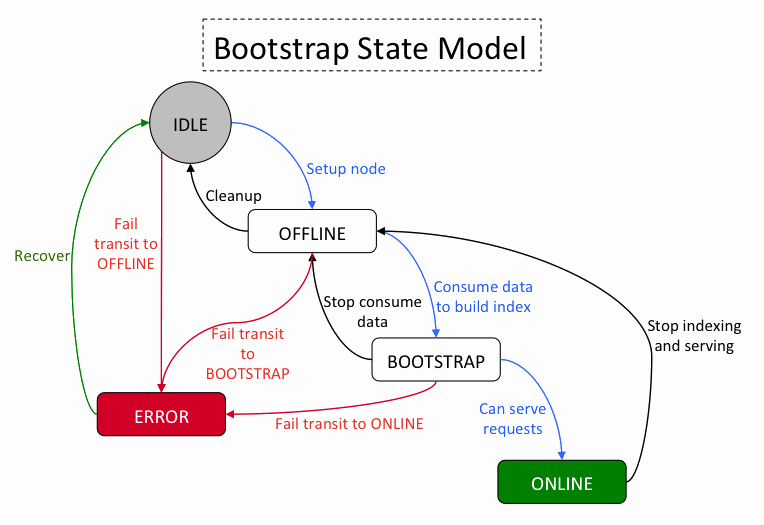
\includegraphics[width=\columnwidth]{bootstrap_statemodel.png}}
    \vspace*{-2ex}
    \caption{\label{fig:bootstrap_statemodel} \seas state machine.}
\end{figure}

Figure~\ref{fig:bootstrap_statemodel} shows the detailed state machine for \seas, another
\helix-managed DDS. As with \\ \ES, the state model and
constraints are configured in \helix. \seas has large number
number of replicas and one of the main optimization goal is to throttle the
maximum number of \\
offline$\rightarrow$bootstrap transitions. 

\subsection{\helix Execution}
%
Thus far we have described how DDSs declare their behavior within \helix.  We
now describe how \helix invokes that behavior on behalf of the DDS at run-time.  
\helix execution is a matter of continually monitoring DDS state and, as
necessary, ordering transitions on the DDS.   There are a variety of changes 
that can occur within a system, both planned and unplanned: bootstrapping the
DDS, adding or losing nodes, adding or deleting resources, adding or deleting
partitions, among others (we discuss detecting the unplanned changes in
Section~\ref{sec:arch}).

\begin{algorithm}
\label{alg:execution}
\caption{\helix execution algorithm}
\begin{algorithmic}[1]
\REPEAT
\STATE validTrans = $\emptyset$
\STATE inflightTrans = $\emptyset$
\FOR {each partition $p_i$}
  \STATE Read currentState
  \STATE Compute targetState 
  \STATE Read $p_i$ pendingTrans
  \STATE inflightTrans.addAll(pendingTrans)
  \STATE requiredTrans = computeTrans(currentState, targetState, 
pendingTrans) 
  \STATE validTrans.addAll(getValidTransSet( \\ requiredTrans))
\ENDFOR
\STATE newTrans = throttleTrans(inflightTrans, validTrans) 
\UNTIL {newTrans == $\emptyset$}
\end{algorithmic}
\end{algorithm}

\eat{%%%%%%%%%
\begin{algorithm}
\label{alg:changeset}
\caption{getPrioritizedValidTransitionSet algorithm.}
\begin{algorithmic}
\STATE pending = $\emptyset$
\STATE Sort requiredTransitions descending by priority
\STATE \FOR {each transition $t_i$ in sorted list}
\STATE \IF (! isViolated(pending, $t_i$)) 
\STATE 	pending.add($t_i$)
\STATE \ENDIF
\STATE \ENDFOR
\end{algorithmic}
\end{algorithm}

\begin{algorithm}
\label{alg:throttle}
\caption{Throttled transition execution.}
\begin{algorithmic}
\STATE FILL THIS IN
\end{algorithmic}
\end{algorithm}
}%%%%%%%%%%%%%

\eat{%%%%%%%%
\begin{algorithm}
\caption{\helix execution algorithm, run anytime a cluster becomes invalid.}
\begin{algorithmic}
\STATE //Compute all transitions
\FORALL {partitions $p_i$}
	 \STATE initialize transition set $T(p_i)=\{\}$
         TODO: write how we compute transitions
\ENDFOR
\STATE //Create per-partition batches
\STATE //Parallel execute batches with optional throttling
\end{algorithmic}
\end{algorithm}
}%%%%%%%%

The most crucial feature of the \helix transition algorithm is that it is identical 
across all of these changes and across all DDSs!  Else, we face a great deal of
complexity trying to manage so many combinations of changes and DDSs, and lose
much of \helix's generality.   
The execution algorithm appears in Algorithm~\ref{alg:execution} and we now step
through it.


In lines 2-3 we initialize two transition sets: validTrans and
inflightTrans, whose purposes we describe shortly.  
The first step, in lines 5-6, is on a partition-by-partition basis, to 
read the DDS's current state and compute a target state, where
target state is a distribution of a partition's replicas over cluster nodes 
that respects the DDS's constraints and optimization goals.  Most of the time, 
the current state will match the target state, and there is nothing to do; they
disagree only when the cluster changes (e.g. nodes lost, partitions added,
\etc).

By default we use the RUSH~\cite{honicky04} algorithm to produce the target state,
though with enhancements to ensure we meet state machine constraints and to
ensure we meet our optimization goals.  Default RUSH relies on
random hashing of a huge number of partitions to meet load balancing goals.
Since DDSs can have as few as 10s of partitions per node, to avoid load skew and
so better meet optimization goals, we
additionally assign each node a budget that limits the number of partitions it
may host.  \helix makes it easy to plug in other algorithms; we
discuss this more in Section~\ref{sec:placement}.

Given a partition's target state, line 7-9 reads all pending transitions for the
partition and then computes necessary additional replica transitions.
Given current state and the state model, producing the set of all necessary
transitions is straightforward
and we omit the details.


The next part of the algorithm computes a set of valid transitions for the
partition, taking into account the already pending transitions and those that
still must occur. The main objective of computing the set of valid transitions is to maximize the 
transitions that can be done in parallel without violating the state constraints. 
Suppose we have $T$ possible transitions for a partition. Note that the maximum
possible value of $T$ is the number of replicas. If \helix issues all these transitions in parallel,
 they can be executed in any order.
To ensure correctness in the DDS, \helix needs to evaluate the system state
for all $T!$ possible orders in which the transitions are executed. The cost of evaluating
the state correctness for $T!$ permutations is exponential in the number of replicas. 
\helix avoids the exponential time complexity by utilizing the fact that
system constraints are expressed in terms of state, which means \helix needs to 
get the count for each state at every intermediate stage.
 In other words, from \helix's point of view, (Node1:Master, Node2:Slave) is no
 different from (Node2:Master, Node1:Slave), since the count of masters and
slaves is 1 each in both cases.

Our solution is to produce valid \emph{transition sets}; for a given
partition, a transition set is valid if
for every possible ordering of its transitions, the partition remains valid.    
Line 10 calls a method getValidTransSet that initializes a
transition set to include all
currently pending transitions for a partition and greedily adds other required
transitions, as long as the transition set remains valid, until no more
transitions can be added.  It considers the transitions in priority order,
according to the optimization goals given by the DDS.

Note we compute transition sets partition-by-partition.  Since the AFSM is
per-partition, we can safely execute a valid transition set per each partition
without making any partition invalid.  Thus, we have two potential dimensions for
parallelism: by building transition sets per partition, and across partitions.

By line 12 we have a set of valid transitions to run
across all partitions.  We do not simply execute them all, but instead now take
into account the DDS's throttling optimization goals.  The throttleTransitions
method takes the set of all inflight transitions (from prior rounds) and then
selects as many additional transitions as possible, without violating
constraints.  Notice that any non-scheduled valid transitions are essentially
forgotten and are considered anew in later rounds.

Finally, not shown in the algorithm is what happens when transitions complete.
We are notified by callback and remove those transitions from their partitions
lists of pending transitions.

The execution algorithm has two greedy key steps, to produce valid transitions and to
choose transitions for execution, rather than deriving both in a single
optimization.
While we could combine the two to produce a provably optimal solution, for the
time being, we find the current approach produces a high level of parallelism,
with highest priority transitions scheduled early.

\subsubsection{\helix Modes of Execution}
\label{sec:placement}
%
By default \helix places replicas using modified RUSH, as described in
Algorithm~\ref{alg:execution}.  
While this approach makes things very simple for some applications, it may not
be powerful enough for all applications, such as those that want to customize
placement of a single resource's partitions or even control placement of
multiple resources' partitions. 

\helix supports 3 different execution modes which allows application to explicitly control the placement and state of the replica.

The default execution mode is \emph{AUTO}, in which \helix decides both the placement and state of the replica. This option is useful 
for applications where creation of a replica is not expensive. A typical example is evenly distributing a group of tasks 
among the currently alive processes. For example, if there are 60 tasks and 4
nodes, \helix assigns 15 tasks to each node.  When one node fails \helix
redistributes its 15 tasks to the remaining 3 nodes. Similarly, if a node is added, \helix 
re-allocates 3 tasks from each of the 4 nodes to the 5th node. \helix does the coordination of 
handing off a task from one node to another and ensures that a task is not
performed by two nodes at any given time. The RUSH algorithm allows us to balance the tasks without having to 
 reshuffle all task assignments. \databus consumer grouping uses this mode of execution.

The second \helix mode is \emph{SEMI-AUTO}.  The DDSs decide the replica placement while \helix still chooses 
the state of those replicas. This is used where creation of additional replica
is expensive, as is typical in DDSs that have a large amount of data associated with each replica. 
The assumption here is that when a node fails, instead of remapping replica placement 
 among the remaining nodes, only the states of replica changes. For example,
 in \ES, when a master fails, \helix promotes a slave to master instead of
 creating a new replica. This ensures mastership transfer is fast,  without negatively impacting
availability of the DDS. \helix provides a way for application to reuse the RUSH algorithm and
ensure that when a node fails, masterships are transferred evenly among
the remaining nodes. \ES uses this mode of execution. As a second example, 
HBase can use \emph{semi-auto} placement to co-locate its regions servers with the HDFS blocks
containing those regions' data.

\helix offers a third mode called \emph{CUSTOM}, in which DDSs completely control the placement and state of each replica. In this 
case \helix does the coordination to move the DDS from its Current state to the Final state expressed by the DDS. 
\helix provides a special interface with which the application provides such
custom functionality when there are changes in the cluster.
This functionality can reside on any of the nodes and \helix ensures that it is
executed on only one node elected as a leader in the DDS. This mode is useful
for applications if it wants to coordinate across multiple resources or have additional logic to
be used to decide the final state of the replicas. It is important to note that
the DDS need only express the final placement and state of replicas; \helix
still computes the transitions needed and executes them ,such that constraints are not violated. This allows 
application to still use the other features of \helix like throttling, pluggable FSM \etc. \seas uses this mode of execution. 
Having this feature also allows \ES to be configured differently based on the
replication channel. At \linkedin we have deployed \ES in production using
native \mysql replication.  One of the requirements for \mysql replication 
is that the replicas of all resources hosted on any node be in the
same State (Master or Slave).
With \emph{CUSTOM} execution \helix lets \ES control the state of all replicas 
across multiple resources to change the state atomically.

Applications may want this varying degree of control either because they are very specialized or because they
are wary of handing over all control to \helix.   We do not want to turn away
such applications, and so permit customized placement in \helix, while allowing
them to benefit from all of \helix's other features, rather than 
force such applications to build their own cluster management from scratch.


%\begin{figure*}[t]
%{\includegraphics[width=0.9\textwidth]{figs/execution_example.png}}
%\caption{Example of \helix execution algorithm.}
%\end{figure*}

\subsubsection{Execution example}
%
We consider a case when a node is added to already existing
cluster to illustrate the execution sequence in Helix.
Suppose we start with an \ES cluster with 3 nodes $n_0 \ldots n_2$, 12
partitions $p_0 \ldots p_{12}$, and a replication level of 3; there are 12 total
replicas per node.  We then add a node $n_3$. 
Intuitively, we want to rebalance the cluster such that every node is left with
9 replicas.  In \helix execution we first compute a target state for each
$p_i$.  For 9 of 12 partitions the target state differs from the current state.  In
particular, 3 partitions get mastered on the new node and 6 partitions get
slaved on the new node.  We compute the required transitions for each partition.
Suppose $p_{10}$ will have its master replica moved from $n_1$ to $n_3$.  $n_1$
must execute $t1=(M \rightarrow S$) for $p_{10}$, while $n_3$ must execute $t2=(O
\rightarrow S)$ and $t3=(S \rightarrow M)$.  We cannot, however, execute these
transitions all in parallel since some orderings make the system invalid.
In order to avoid $p_{10}$ being mastered twice, $t3$ must execute only after
$t1$ completes. Helix automatically enforces this since it
issues a transition if and only if it does not violate any of the
state constraints. There are two possible valid groupings to reach this target
state. One is to execute $t1$ and $t2$ in
parallel, and then execute $t3$, while the other is to execute $t2$, $t1$, and $t3$
sequentially. Helix chooses
the first approach.
 
Across all partitions, we produce
a set of 18 valid transitions that we can execute in parallel; however, since 
this \ES cluster prohibits more than 10 from running in parallel, 
we produce a transition set of size 10, and save all remaining transitions
(delayed due to validity or throttling) to later rounds. Its important to note that
Helix does not wait for all 10 transitions to complete before issuing the
remaining transitions. Instead, as soon as the first transition is completed, it
reruns the execution algorithm and tries to issue additional transitions. 

\eat{%%%%%%%
that makes transition decisions is identical across all
DDSs.  Faced with all these changes, \helix uses the DDS-provided AFSM to
first check whether the DDS is in a valid configuration and second, if not, initiate transitions to
make it valid.  These two steps constitute a tight feedback look that \helix
executes until the DDS is valid.

Since partitions are the DDS's lowest level of state granularity and are
mutually independent, \helix runs the execution algorithm against each partition
separately.  The execution algorithm is as follows:
}%%%%%%%%%




\eat{%%%%%%%%
\helix supports constraints at multiple granularities. 
Partition
Resource
Node
Cluster
These constraints can be applicable either to a STATE or a TRANSITION.
This feature of being able to specify constraint at various granularities is
proven to be quite useful to achieve important requirements such as
partition placement, throttling, load balancing etc. 
}%%%%%%%%%%%%%

\eat{%%%%%%%
Before we describe how these constraints can be used to
solve system specific requirements, lets recap the two important things need to
happen in \helix given an AFSM
1) Compute the Partition,State to Node mapping such that constraints will be satisfied. 
2) Once the mapping is computed, issue transitions to the nodes such that constraints are not violated.
Now lets see how Helix achieves these two functionalities
\subsubsection{Partition Mapping Module}
\label{sec:partitionmappingmodule}
Apart from satisfying simple constraints on the state machine such as
Number of Master=1, Number of Slaves=3 there can be more constraints that this
assignment needs to satisfy.
For example, as we see in Espresso use case, the assignment has to satisfy the 1) Master partitions are
evenly distributed among the nodes 2) (1) has to hold good even after nodes
fail/add.
}%%%%%%%%%%%%

\eat{%%%%%%%%
Helix automatically comes with few generic assignment algorithms that solves
most of the assignment problems. It supports multiple modes
1) Auto: In this mode the (partition,state) -> (Node) assignment is automatically
calculated for every change in the cluster state. Lets
consider the requirements of Espresso to distribute Master Partitions
equally among the nodes in the cluster. This constraint can be provided to
Helix as max number of master partitions per node=Total number of
partitions/Alive Nodes. This constraint ensures that the
(partition,state)->(node) solution computed by Helix solves requirement 1) and
2).
Another interesting but quite useful that automatically comes with Helix is it tries to minimize the transitions required in the system to reach the stable state. 
There are two interesting cases to that will make explain this in detail. When a
master fails there are two solutions possible. 
Node Failure:
One is to promote a partition
which is currently in Slave state for that partition. The other solution is to
assign this partition to a new node. Helix automatically chooses the first
solution since it requires the minimum transition. This is achieved by
specifying the following constraints.
a Max partition per node = Total partition*Number of Replicas/Nodes. 
b) Number of Slaves is between 0 and 3.
The denominator of this constraint a) is very important, what this means is once
the partition->Nodes mapping is computed it never changes until new nodes are added
to the system. This is very important to stateful data
systems like Espresso where creation/removal of a partition is expensive. Constraint b) is provided so that Helix knows that system can
be stable with less number of slaves. Lets say that Espresso has to change
this behavior in future such that new replicas are automatically created all it
needs to do is change is 
a) Max partition per node=(Total partition*Number of Replicas)/Alive Nodes. 
b) Number of Slaves is 3.

Node addition
New nodes are added to system to handle more load, this is simple way to
scale the system since some partitions now can be hosted on the new nodes. One
problem is here what partitions should be moved to the new nodes. This operation
generally known as rebalancing is often not thought of carefully in most DDS.
This operation ends up being very expensive, manual and laborious. Helix provides
three important features here, automation, throttling and minimizing partition
shuffling and downtime. Automation comes
naturally because of the state machine approach. The algorithm that computes the
assignment of partition,state-> node automatically tries to minimize the number of
transitions required to system from current state to new state.  Downtime can be
minimized by prioritizing transitions. In case of Espresso, when new node(N2) is
added and it is supposed to become Master for Partition P1 which is currently
mastered at N1. The followings transitions need to happen on P1.
t1 N1 -> M-S 
t2 N2 ->O-S
t3 N2-> S-M

There are two ways these transitions can be fired in multiple groups. 
t1, t2 and then t3
t2 and then t1 and then t3

If all transitions take equal amount of time then first solution is faster since
t1 and t2 can happen in parallel and t3 can be fired as soon as t1 and t2 is
completed. Though this solution looks attractive, it will result in larger
downtime since O-S generally takes more time since it has to do bootstrap of P1
which might involve copying large data. This can be easily achieved in Helix by
prioritizing the transitions. For example, prioritizing transitions in order of
S-M, O-S, M-S will ensure that downtime is minimum. <K>(Need to verify this)<K>

Another important thins needed in distributed system but often ignored until a
catastrophe is throttling. For example, when new nodes are added there will be
massive amount of bootstrapping that will move data around in the system. This
process if not controlled can bring down the entire cluster.
One can simply make use of this feature by saying
Max offline to slave transition per node=3.
max offline to slave transition in cluster=10
It is important to have the ability to specify the constraints at multiple
granualarities based on the system capacity.

 
 
3) Custom: We have seen that most cases the Auto mode is sufficient, but
in some cases system might have their own custom logic to decide the
(partition,state)->(node) assignment. In these cases, Helix supports Custom mode
where the application can plugin their custom code to dictate the
assignment.Custom mode simply means that Assignment is provided externally,
Helix still does the heavy lifting of issuing the transitions and ensuring
constraints on State are not violated and transition constraints are satisfied.
\aes{This section is missing, need to fill this in.}
\aes{This section must talk about how this works when we have load-imbalance due
to skew or whatever.  If you knew weights of partitions have changed, what do
you do?  \helix must observe this (through monitoring) and then act.}
}%%%%%%%%%%%%%



\subsection{Monitoring and Alerts}
\label{alerts}
%
\helix provides functionality for monitoring cluster \\ health, both for the sake
of alerting human operators and to inform \helix-directed transitions.  
For example, operators and \helix may be want to monitor request throughputs and 
latencies, and at a number of granularities: per-server, per-partition, 
per-customer, per-database, etc.  These metrics help systems detect if they are 
meeting or missing latency SLAs, detect imbalanced load among servers 
(and trigger corrective action), and even detect failing components.  

Ultimately, the DDS, rather than \helix, should choose what to montitor.  \helix
provides a generic framework for monitoring and alerting.  The DDS submits
statistics and alert \emph{expressions} they want monitored to \helix and then
at run-time emit statistics to \helix that match those expressions.  \helix is
oblivious to the semantic meaning of the statistics, yet receives, stores, and
aggregates them, and fires any alerts that trigger.  In this paper we do not
fully specify the framework, but instead give a few examples of its
expressiveness and how it is used.

\helix stats follow the format
\texttt{(aggregateType)(statName)}.
For example, a system might create \\
\texttt{window(5)(db*.partition*.reqCount)} \\
We use \emph{aggregation types} to specify how stats should be maintained over time.  
In this case, the aggregation type is a window of the last 5 reported values.
This stat uses wildcards to tell \helix to track request count for every partition of 
every db.  We also provide aggregate types \emph{accumulate}, which sums all values 
reported over time and \emph{decay}, which maintains a decaying sum.

\helix can maintain stats for their own sake; they are also a building block for
alerts.  An example alert is: \\
\texttt{decay(0.5)(dbFoo.partition10.reqCount) > 100} \\
\helix fires an alert if the time decaying sum of request counts on 
dbFoo's partition 10 exceeds 100.  Similarly, we can instatiate multiple
alerts at once using wildcards: \\
\texttt{decay(0.5)(dbFoo.partition*.reqCount) > 100} \\
The aggregator outputs a column of request counts and an alert fires 
for \emph{each} value
above 100. 

Alerts support simple stats enumeration and aggregation using 
\emph{pipeline operators}.
\eat{%%%%%%  
Pipelined alerts follow the format: \\
$(aggregateType)(s_1, s_2 \ldots s_m)|o_1|o_2| \ldots |o_n$. \\
$s_i$ indicates a stat name and $o_j$ indicates an operator.  An aggregator
ouputs a column of values for each $s_i$.  
}%%%%%%%%
Each operator expects tuples with 1 or more 
input columns and outputs tuples with 1 or more columns (valid number of input columns is
operator specific).  
%A simple example is: \\
%\texttt{decay(0.5)(dbFoo.partition*.successCount, \\
%dbFoo.partition*.failureCount)$|$SUM) \\ > 100} \\
%For each dbFoo partition, this alert sums the success and failure
%counts, deriving a request count, and
%fires if that sum exceeds 100. 
An example aggregating alert is: \\
\texttt{decay(0.5)(dbFoo.partition*.failureCount, \\
dbFoo.partition*.reqCount)$|$SUMEACH$|$DIVIDE) > 100} \\
This alert sums failure counts across partitions, sums request counts
across all partitions, and divides to generate a
database-wide failure rate.

The sets aggregator and operator types within \helix are themselves easy to
expand.  The only requirement in adding an aggregator is that pipeline operators
and comparators (">" in above example) must be able to interpret its output.
Pieline operators must specify their required number of input and output columns.  This
lets users apply arbitrary operator chains, since \helix can determine in
advance whether those chains are valid.  While have implemented a number of
operators, the most commonly used for simple aggregations are SUMEACH, which
sums each input column to produce an equal number of singleton columns, and SUM,
which does row-wise summing. 

\eat{%%%%%%%
\subsection{older outline}
Design
  -Design is generic, but use 2 driving examples as running examples.
  -Justify any interesting design decisions, and the theme is to emphasize how they help Helix be generic.
  -Think about giving anecdote about how we easily spun Espresso w/mysql replication from Espresso w/databus replication.  Repeat this in evalation.

Limitations/negatives
 -What are the possible problems?
 -Why aren't we worried about them right now?
 -What are possible solutions if we want to address them.


Note about ideal state terminology.
-We want to describe the set of constraints and optimization goals as 1 thing, and an actual config that achieves those goals as a 2nd thing.
-The first thing can be described as an optimization problem: maybe "optimization spec?"
-The second thing is a solution: maybe "assignment"

Consider merged impl with this section if it makes sense
}%%%%%%%%%

\eat{%%%%%%%%
%
\helix relies on Zookeeper for detecting hard failures (e.g. a lost server).  Distributed data stores need much more nuanced monitoring as well, however.  Some typical key metrics are request throughputs and latencies, and we monitor these at a number of granularities: per-server, per-partition, per-customer, per-database, etc.  These metrics help systems detect if they are meeting or missing latency SLAs, detect imbalanced load among servers (and trigger corrective action), and even detect failing components.  

\helix provides a generic statistics monitoring and alerting framework.  Systems submit statistic and alert \emph{expressions} they want monitored to \helix and then emit 
specific statistics matching these expressions during operation.  \helix
receives, stores and aggregates statistics and evaluates them against alerts,
firing those that have triggered.  The stats format is purposefully general so
that systems can monitor whatever metrics they want at whatever granularity.
The onus is on the system to emit stats that match its expressions.  \helix
stats have the format: \\
\texttt{(aggregateType)(statName)} \\
For example, a system might create: \\
\texttt{window(5)(db*.partition*.reqCount)} \\
We use \emph{aggregation types} to specify how stats should be maintained over time.  In this case, the aggregation type is a window of the last 5 reported values.
This stat uses wildcards to tell \helix to track request count for every partition of every db.  We currently support two other aggregate types: \emph{accumulate}, which sums all values reported over time, and \emph{decay}, which maintains a decaying sum.

It is possible to maintain stats for their own sake or to use them as building blocks for alerts.  An example alert on request count is: \\
\texttt{decay(0.5)(dbFoo.partition10.reqCount) > 100} \\
This indicates \helix should fire an alert if the time decaying sum of request counts on dbFoo, partition 10 rises above 100.  We can also use wildcards to instantiate 
multiple alerts as follows: \\
\texttt{decay(0.5)(dbFoo.partition*.reqCount) > 100} \\
This alert is identical to the previous, but now the aggregator outputs a \emph{column} of request count values, one for each dbFoo partition, and creates an alert for each partition.

\helix alerts also support simple stats enumeration and aggregation before alert evaluation using \emph{pipeline operators}.  Pipelined alerts follow the format: \\
$(aggregate_type)(s_1, s_2 \ldots s_m)|o_1|o_2| \ldots |o_n$. \\
$s_i$ indicates a stat name and $o_j$ indicates an operator.  Stats aggregation as before outputs columns of values.  Operators expect some 1 or more input data columns and output 1 or more data columns.  A simple example is: \\
\texttt{decay(0.5)(dbFoo.partition*.successcount, dbFoo.partition*.failurecount)|EXPAND|SUM) > 100} \\
This alert identifies each dbFoo partition, sums their success and failure counts, and alerts if that sum exceeds 100 for any partition. 
Finally, we provide a more complex aggregation: \\
\texttt{decay(0.5)(dbFoo.partition*.failurecount, dbFoo.partition*.reqCount)|EXPAND|SUMEACH|DIVIDE) > 100} \\
This alert sums all failure counts, sums all request counts, and then uses division to generate a failure rate.

We have made aggregation types and pipeline operators pluggable.  Aggregation types are flexible, but pipeline operators and comparators (\">\" in above examples) must be able to interpret the stat.  Pipeline operators are also flexible, but must specify valid values for the number of input columns it expects and output columns it generates; \helix allows for arbitrary chaining of operators, as long as each step produces a valid number of columns for the next step.  That is, if operator $o_j$ requires a number of input columns from $I(o_j)$ and generates a number of output columns in $O(o_j)$, then we require $I(o_j) \in O(o_{j-1})$ and $I(o_{j+1}) \in O(o_j)$.  For example, \texttt{SUM} takes 1 or more input columns and outputs 1 columns.  These constraints make it easy to expand the set of operators, without worrying about compatibility with existing ones.

\aes{optional, provide a table of all implemented agg types and pipeline operators}
\aes{formally define pipelines?}
\aes{describe taking action on alerts...disabling partitions or servers}
}%%%%%%%%%%%

\section{Helix Architecture}
\label{sec:arch}
%

Section~\ref{sec:design} describes how \helix lets a DDS specify their model of
operation and then executes against it.  This section presents the \helix system
architecture that implements these concepts.

\begin{figure}
%\fbox{
\begin{minipage}[t]{0.48\textwidth}
%\centering
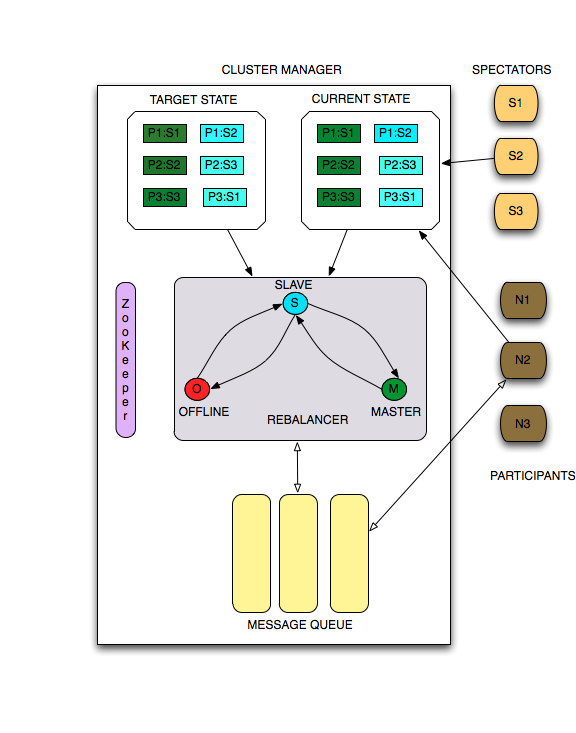
\includegraphics[width=0.95\textwidth]{Helix.png}
%\vspace*{-4ex}
\caption{Helix Architecture}
\label{fig:arch}
\end{minipage}
%}
\end{figure}

\subsection{\helix Roles}
\label{sec:roles}
%
\helix implements three roles, and each component of a DDS takes on at least one of them.
The \emph{controller} is a pure \helix component.  It hosts the state machine engine, 
runs the execution algorithm, and issues transitions against the DDS.  It is the
core component of \helix.

The DDS's nodes are \emph{participants}, but run the \helix library.  The
library is responsible for invoking callbacks whenever the controller initiates
a state transition on the participant.  The DDS is responsible for implementing
those callbacks.  In this way, \helix remains oblivious to the semantic meaning
of a state transition, or how to actually implement the transition.  For
example, in a \emph{LeaderStandby} model, the DDS implements methods
\emph{OnBecomeLeaderFromStandby} \\ and \emph{OnBecomeStandbyFromLeader}.

The \emph{spectator} role is for DDS components that need to observe system
state.  Spectators get notification anytime a transition occurs.  A typical
spectator is the router component that appears in data stores like \\ \ES.  The
routers must know how partitions are distributed in order to direct client
requests and so must be get up-to-date with any partition moves.  The routers do
not store any partitions themselves, however, and the controller never executes
transitions against them.

The roles are at a logical level.  A DDS may contain multiple instances of each
role, and they can be run on separate physical components, run in different
processes on the same component, or even combined into the same process.
 
Dividing responsibility among the components brings a number of key
advantages.  (A) All global state is managed by the controller, and so the DDS can
focus on implementing only the local transition logic.  (B) The participant need
not actually know the state model the control is using to manage its DDS, as long as all the
transitions required by that state model are implemented.  
For example, we can move a DDS from a MasterSlave model to a read-only SlaveOnly
model with no changes to participants.  The participants will simply never
be asked to execute slave$\rightarrow$master transitions.  (C) A
central decision maker avoids the complexity of having multiple components come
to consensus on their roles.    

\subsection{Connecting components with Zookeeper}

Given the three \helix components, we now describe their implementation and how
they interact. \\ Zookeeper~\cite{zookeeper} plays an integral role in this aspect
of \helix.

The controller needs to determine the current state of the DDS and detect
changes to that state, \eg node failures.  We can either build this
functionality into the controller directly or rely on an external component that
itself persists state and notifies on changes. 
When the controller chooses state transitions to execute, it must reliably
communicate these to participants.  Once complete, the participants must
communicate their status back to the controller.  Again, we either build a custom
communication channel between the controller and participants, or rely on an
external system. 
The controller cannot be a single point of failure; in particular, when the
controller fails, we cannot afford to lose either controller functionality or
the state it manages.

\helix relies on Zookeeper to meet all of these requirements.  We utilize
Zookeeper's group membership and change notification to detect DDS state
changes.  Zookeeper is
designed to maintain system state, and is itself fault tolerant.  By storing
all the controller's state in Zookeeper, we make the controller itself stateless
and therefore simple to replace on a failure.  
 
We also leverage Zookeeper to construct the reliable communication channel
between controller and participants.  
The channel is modeled as a queue in Zookeeper and the controller and
participants act as producers and consumers to this queue. Producers can
can send multiple messages through the queue and consumers can process the messages in parallel. 
This channel brings side operational benefits like the ability to cancel
transitions and to send other command messages between nodes.

Figure~\ref{fig:arch} illustrates the \helix architecture and brings together
the different components and how they are represented in Zookeeper.  
The diagram is from the controller's perspective.  The AFSM is specified by each
DDS, but is then itself stored in Zookeeper.  We also maintain the current
states of all partition replicas and target states for partition replicas in
Zookeeper.  Recall that any differences between these states trigger the
controller to invoke state transitions.  These transitions are written to
the messaging queue for execution by the participants.  Finally, \helix
maintains a list of participants and spectators in 
Zookeeper as \emph{ephemeral nodes} that heartbeat with Zookeeper.  If any of
the nodes die, Zookeeper notifies the controller so it can take corrective
action.

\eat{%%%%%%%%%
As shown in Figure ?, We maintain the following state in Zookeeper.

\begin{itemize}
\item \emph{Target State} The target state of a resource in the cluster is stored as a znode in Zookeeper.
\item \emph{Current State} The current state of partitions of the resource on a participant is stored in a znode.
\item \emph{Message Queue} A message queue between the controller and every participant in the cluster is stored in a znode.
\item \emph{Live Instances} Every participant in the cluster creates an ephemeral znode in Zookeeper. This znode gets removed by Zookeeper if the node fails and stopped communicating a heartbeat to Zookeeper.
\end{itemize}

The controller maintains a watch on \emph{Live Instances}, \emph{Target State}, \emph{Current State} and \emph{Message Queue}. It responds to changes in \emph{Live Instances}, \emph{Target State}, \emph{Current State} and executes the state transition algorithm to achieve the \emph{Target State} of the cluster.

For example, when a new node is added to the cluster, Helix recomputes the \emph{Target State} of the cluster to assign some of the partitions on to the new node. Once the \emph{Target State} is specified, the controller is notified and it computes the state transitions to go from \emph{Current State} to \emph{Target State}. After applying the constraints defined on the state model and optimization goals, a  subset or all of the state transitions are then enqueued into the \emph{Message Queue} of the appropriate participant nodes. The participants watch their \emph{Message Queue} for messages from the controller. The Helix library in the participant invokes the callbacks supplied by the DDS that correspond to the state transitions. Once the callbacks complete successfully, the Helix library in the participant updates the \emph{Current State}.
}%%%%%%%%%%%%%

\subsection{DDS Integration with \helix}
This section describes how a DDS deploys with \helix.
The DDS must provide 3 things.

\noindent \textbf{Define Cluster}
The DDS defines the physical cluster and its physical nodes.  \helix provides an
admin API, illustrated here: 
\small\begin{verbatim}
helix-admin --addCluster EspressoCluster 
helix-admin --addNode EspressoCluster <esp10:1234>
\end{verbatim}
\normalsize

\noindent \textbf{Define Resource, State Model and Constraints}
Once the physical cluster is established, the next step is to logically add the
DDS, including the state model that defines it and the resources it will supply.
Again, \helix provides an admin API: 
\small\begin{verbatim}

  helix-admin --addStateModel MasterSlave states=<M,S,O> 
              legal_transitions=<O-S, S-M, M-S, S-0> 
              constraints="count(M)<=1 count(S)<=3" 
  helix-admin --addResource 
             clusterName=EspressoCluster
		     resourceName=EspressoDB numPartitions=8 
		     replica=3
		     stateModelName=MasterSlave
\end{verbatim}
\normalsize


Given the above admin commands, \helix itself computes an initial target state
for the resource: 
\small\begin{verbatim}
{
  "id" : "EspressoDB",
  "simpleFields" : {
    "IDEAL_STATE_MODE" : "AUTO",
    "NUM_PARTITIONS" : "8",
    "REPLICAS" : "1",
    "STATE_MODEL_DEF_REF" : "MasterSlave",
  },
  "mapFields" : {
    "EspressoDB_0" : { "node0" : "MASTER",
                       "node1" : "SLAVE"  },
    "EspressoDB_1" : { "node0" : "MASTER",
                       "node1" : "SLAVE"  },
    "EspressoDB_2" : { "node0" : "SLAVE",
                       "node1" : "MASTER" },
    "EspressoDB_3" : { "node0" : "SLAVE",
                       "node1" : "MASTER" },
  }
}
\end{verbatim}
\normalsize

\noindent \textbf{Implement Callback Handlers}
The final task for a DDS is to implement logic for each state transition encoded
in their state machine.  We give a partial example of handler prototypes for
\ES's use of MasterSlave.

\small\begin{verbatim}
EspressoStateModel extends StateModel
{
 void offlineToSlave(Message task,
     NotificationContext context)
 {
  // DDS Logic for state transition
 }
 void slaveToMaster(Message task,
     NotificationContext context)
 {
  //DDS logic for state transition
 }
}
\end{verbatim}
\normalsize
\subsection{Scaling \helix into a Service}

\eat{%%%%%%%%
We carefully divided up \helix's responsibilities
between the controller and participant roles and, in doing so, gain a number of
advantages.

\begin{itemize}

\item  The participant remains completely unaware of the DDS's
global state.   This makes the job of developers implementing the DDS specific
logic considerably simpler; they only need to write the node's local transition
logic. The responsibility of maintaining the distributed system and responding
to changes in that global state is solely with the controller, which DDS
developers need not touch.
 
\item Since the participant is unaware of global state is
that the same DDS can easily be configured differently for different use cases.
Consider key-value storage systems, which typically support reads and writes,
but sometimes are deployed as read-only (with data periodically bulk loaded).
In the former case, we might use a MASTER-SLAVE state model, and in the latter,
a MASTER-only (or SLAVE-only) mode, since there is no need to differentiate
replicas.  In both cases, the participant code does not change, and the
participants are in fact oblivious to what state model is invoked. 

\item Having a central controller component with global system state simplifies
transition decision-making.  An alternative approach followed by many distributed systems
is to divide responsibility for decisions among the participants.  Consider the
LeaderStandby state model.  A single participant per partition serves as Leader
at any given time.  In the absence of a controller, participants use a central
lock manager to coordinate leader election; when the current leader fails, the
first participant to acquire the lock becomes the new leader.  In large systems with many partitions
this can lead to a herd effects that can be detrimental to performance. 

\item Multiple participants simultaneously making decisions based on global state increases the chance of \emph{Split Brain} problem where multiple participants make conflicting decisions about the global state of the cluster.

\end{itemize}
}%%%%%%%%%

%\subsubsection {Scaling the controller}
The risks of having a single controller as we have described so far is that it
can become a bottleneck or a single source of failure (even if it is easy to
replace).  We now discuss our approach for distributing the controller that
actually lets Helix provide cluster management as a service. 

To avoid making the controller a single point of failure, we deploy multiple
controllers. A cluster, however, should be managed by only one controller at a time. 
This itself can easily be expressed using a LeaderStandby state model with the constraint 
that every cluster must have exactly one controller managing it! Thus we set up multiple 
controllers as a participants of a \emph{supercluster} comprised of the different clusters 
themselves as the resource. One of the controllers manages this supercluster. If that controller 
fails, another controller gets selected as the Leader for the supercluster. This
guarantees that each cluster has exactly one controller.  

The supercluster drives home \helix's ability to manage any DDS, in this case
itself.  \helix itself becomes a scalable DDS that in turns manages multiple DDSs. 
In practice we typically deploy a set of 3 controllers capable of managing over
50 clusters. 

\eat{%%%%%%%%%
\subsection{OLD STUFF FOR ARCH, BUT CAN PULL TEXT FROM HERE}

\subsection{Supporting no SPOF}
In order for to support this abstraction we need a communication
channel between controller and participant. Its also important that
controller does not become a Single Point Of Failure (SPOF) and
system is stable if any of the component in the system fails. This
means that the state of the system must be durable and also the
communication channel between controller and participant must be able
to handle failures. We use Zookeeper to maintain the state
of the system. Along from being highly available system to store the
cluster state Zookeeper also provides group member ship and also
change notification in cluster state. More info on Zookeeper can be
found at \url{http://zookeeper.apache.org}

\subsection{Stabilizing the system---This should be taken care of by design
section...delete this later}

External changes (Section~\ref{Requirements}) conspire to change the
state of the system, potentially into a less desirable one. The job of
the controller is to restore balance. It does so by defining
\be
\item Current State (CS) --- the current state of the system. The example of
Table~\ref{CS_Example} describes a system with 3 nodes, \(N_1, N_2,
  N_3\), and 4 partitions
such that partition 1 has a replica 
(i) in state \(M\) on \(N_1\)
(ii) in state \(S\) on \(N_2, N_3\)
(iii) in state \(O\) on \(N_4\)
\item Ideal State (IS) --- the final expected state of partition on a 
node. It is re-calculated every time there is a change in the system.  
This is not expressed in terms of an assignment as in
Table~\ref{CS_Example}. Instead, it is expressed in terms of desiderata.
In the example of Espresso (Section~\ref{Espresso}), 
  \be
  \item A partition should not have 2 replicas on the same machine
  \item The maximum number of partitions in state \(M\) on any machine
  should be minimized
  \item \TBC
  \ee
\ee

\begin{table}
\centering
\begin{tabular}{|l|l|l|l|l|} \hline \hline
            & \(N_1\) & \(N_2\) & \(N_3\) & \(N_4\) \\ \hline \hline
State \(M\)       & \(P_1\)  &         &         & \\ \hline 
State \(S\)       &         & \(P_1\) & \(P_1\) & \\ \hline 
State \(O\)       &         &         &         & \(P_1\) \\ \hline 
\end{tabular}
\label{CS_Example}
\caption{Example of Current State}
\end{table}

\subsubsection{Instantiating an IS}
We take the requirements of an IS as input and produce a mapping of X to
Y as an output.

%{\em 
The goal of this algorithm is simple, it
considers all the nodes that are currently up in the cluster and
computes the state for each partition on a given node so that cluster
is stable and all the constraints are satisfied.


Consider a partition and 4 nodes. 
Lets take a simple example of having these constraints.  Number of
partitions 3. Number of nodes 3 Add the example here and compute the
ideal state such that constraints are satisfied. A simple solution is
N1:M N2:S N3:S

Now lets walk through what happens when the nodes are started in the
cluster.

All nodes(N1,N2,N3) start in the Offline state, the ideal state based
on the constraint and live nodes is computed as N1:MASTER, N2:SLAVE,
N3:SLAVE. Another key aspect of the algorithm is parallelize the
transitions without compromising the state constraints. More details
on this algorithm can be found in section

Controller sends OFFLINE-SLAVE transition message to all 3 nodes, as
soon N1 becomes SLAVE, controller issues SLAVE-MASTER transition
message to N1. It wont issue any more transitions after N1 becomes
master because all the constraints of the system are satisfied. Note
that all transitions are issues by consulting the state machine
provided by the application.

Failure:

We will see how the same algorithm is applicable to a Node Failure.
Lets say node N1 fails, then controller re computes the Idealstate as
N2:M, N3:S. Note that controller knows that N1 is down and assigns
MASTER state to N2.  The current state immediately after the failure
is N1:O, N2:S N3:S. It issues S-M transition to N2.

Similarly Node addition, removal and partition addition/removal are
also taken care of in similar fashion.


The role of a spectator is simply be aware of the state changes
happening in the cluster.

Algorithm: Psuedo code Controller gets the Ideal State and the Current
State of active storage nodes from ZK Compute the delta between Ideal
State and Current State for each partition across all participant
nodes For each partition compute tasks based on State Machine
Table. Its possible to configure priority on the state Transition. For
example in case of Espresso, Attempt Mastership transfer if possible
without violating constraint.  Partition Addition Drop Partition[Can
be done when its the only task possible per partition to avoid
complexity] Add the transitions[parallel if possible] to respective
queue for each node.  If a task is dependent on another task being
completed do not add that task.  After any task is completed by
Participant, Controllers gets notified of the change and State
Transition algorithm is re-run until the current state is same as
Ideal State.

Apart from satisfying the state constraints the same algorithm also
takes care of satisfying the constraints on state transition
}%%%%%%%%%%%%



%\section{Additional Features}
\label{section:other}
%
\aes{OWNERS: Ramesh on correctness testing, Kapil on rest}

\subsection{Generic Correctness Testing}
-among other things, mention this testing useful in dev through production

Other Stuff:
-Chaos monkey
-Operability/manageability (TBD)
-Look in misc.tex for removed text that may help here
-

\section{Evaluation}
\label{sec:eval}
%
This section describes our experience running \helix in production at \linkedin and
then presents experiments demonstrating \helix's functionality and production.

\subsection{\helix at \linkedin}
\label{sec:production}
%
From the beginning we built \helix for general purpose use, targeting \ES, \seas
and \databus.  As mentioned earlier, we chose these systems
to ensure \helix became a truly general cluster manager and not, say, a
cluster manager for distributed databases. 
The systems were themselves under development and in need of cluster management
functionality, and so were likewise attracted to \helix.
At the time of this writing, all three of \ES, \seas and \databus run in
production supported by \helix.

With every \helix-DDS integration we found and repaired gaps in the \helix
design, while maintaining its generality.  For example, \seas needed more
control than auto replica placement offers, and so we added semi-auto and
custom modes.
We also added a \emph{zone} concept to support grouping a set of
nodes together.  This is useful, for example, in rack-aware replica placement
strategies.  

The first \helix version did not include constraints and goals on transitions, but instead
satisfied this requirement by overloading state constraints and goals.  This complicated
the algorithms for computing and throttling transitions.  We added support for
transitions to remove this complexity, as well as add support for throttling
transitions at different cluster granularities.

\eat{%%%%%%%
\helix's generic model of a DDS cluster has indeed given us the ability to
greatly accelerate the cluster management aspects of DDS development.  A great
example came from experimenting with different replication designs for \ES.  One
preliminary design we tried was to use native
\mysql-based
replication to synchronize slave replicas with masters, rather than
\databus-based replication.  \aes{briefly explain why mysql-based is not as
good. Kishore: Kapil can you fill this up ?}  

The \ES changes needed to
integrate with \mysql replication took a
considerable amount of time, but the cluster management changes were nearly
trivial.  One change for this version of \ES is that it required each node to contain only masters or only
saves.  We did not have to change its state model but rather only changed its
placement optimization goals to achieve this.  This stresses the value of
\helix's pluggable design. 
A second change was to have each slave-only node in the cluster know its
partitions' masters, in order to initiate replication.  We added no \ES code to
support this communication, but instead simply added the spectator role to each
\ES node.   This shows the value we gain from the \helix roles and being able to
flexibly combine them.
}%%%%%%%%%%

\textbf{DDS debugging and correctness checking}
%
One of the most interesting benefits of \helix falls out of its ability to
manage a cluster without understanding its purpose.  We have built a debugging
tool capable to analyzing a DDS's correctness without understanding its purpose.
Testing distributed systems is extremely difficult and laborious, and it cannot
be done with simple unit tests.   Generic
deubugging tools that function in the distributed setting are especially valuable.  

Our tool uses the ''instrument,
simulate, analyze'' methodology. This consists of
\squishlist
\item \textbf{Instrument} Insert probes that provide information about the state of the system
over time.  We use Zookeeper logs as ''probes.''
\item \textbf{Simulate} We use robots to create cluster error, killing componets
and injecting faults, both on the DDS and \helix sides.
\item \textbf{Analyze} We parse the logs into a relational format, load them into a database as
a set of tables and then write invariants on the DDS's constraints.  Violation
of the constraints signals a possible bug.
\squishend

Every DDS that uses \helix automatically benefits from this tool and it has been crucial
in improving performance and debugging production issues.  
One of the most difficult parts of debugging a DDS is understanding the sequence
of events that leads to failure.  \helix logging plus the debugging tool make it
easy to collect system information and evaluate it.
As a concrete example, the experiment on
planned downtime we describe in Section~\ref{sec:downtime} uses this tool to
measure total downtime and partition availability during software upgrades.
This lets us experiment with different upgrade policies and ensure they are
performant and valid.

\eat{%%%%%%%
One of the most interesting and useful benefits of \helix is its ability to
analyze a DDS's correctness without having any specific knowledge of the DDS's
functionality.  \aes{Ramesh to describe how we have built tools to co-analyze a
log and a state model to check for correctness, how often a DDS is in
violation.}  \aes{Introduce experiment in this area.}  \aes{Show a graph of tool
in practice.}  \aes{Describe result...since this is now in the production
experience section, tone should be how this helps us write/test/deploy DDSs.}
\aes{Make sure to point out that violations do not necessarily mean bugs...just
a little is unavoidable, more than a little could be a design issue, lots could
be a bug.  This tools helps the designer figure gives them insight into DDS so
they can figure it out.}
}%%%%%%%%%%%%

\subsection{Experiments}
\label{sec:experiments}
%
Our experiments draw from a combination of production and experimental
environments, using the DDS \ES.  The clusters are built from
production-class commodity servers.  The details of the production
clusters are confidential, but we present details on our experimental cluster 
throughout our experiment discussion. 

\eat{%%%%%%%
Throughout the experiments we vary different parameters of \helix and
\ES.
We default to the following settings and list changes with each experiment. 
\aes{Kishore to put in a single default value for each param}
\begin{table}
\begin{tabular}{| l | l | }
\hline  Transition Execution Time & 100ms  \\ 
\hline  Replicas & 3 \\
\hline
\end{tabular}
\end{table}
}%%%%%%

\subsubsection{Bootstrap}
\label{sec:bootstrap}
%

\begin{figure*}[t]
  \begin{minipage}[t]{0.48\textwidth}
    {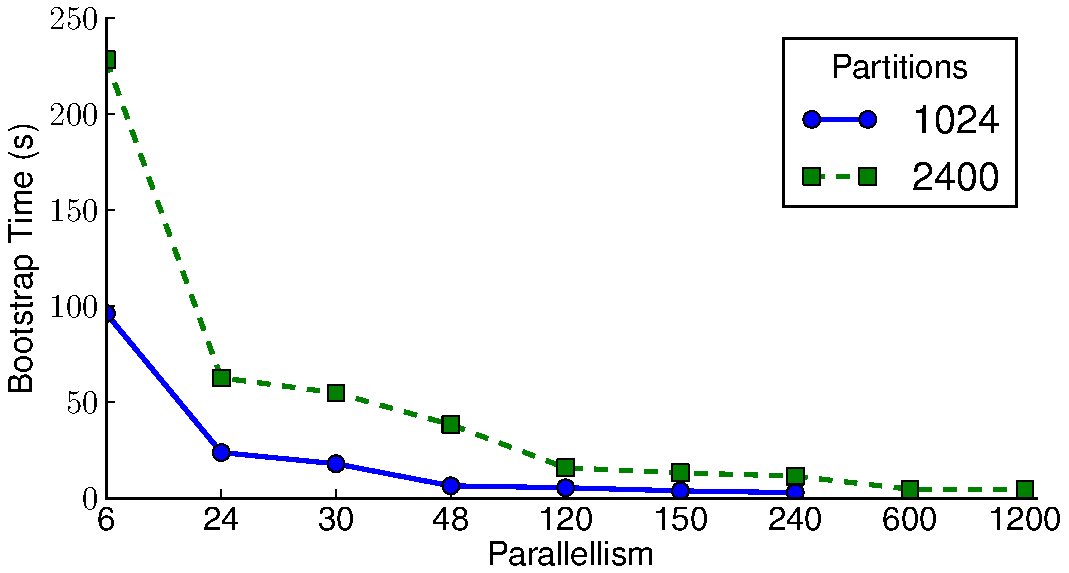
\includegraphics[width=0.90\textwidth]{bootstrap.pdf}}
    \vspace*{-2ex}
    \caption{\label{fig:bootstrap_time} \ES transition parallelism vs. bootstrap time.}
  \end{minipage}
  \hfill
  \begin{minipage}[t]{0.48\textwidth}
    {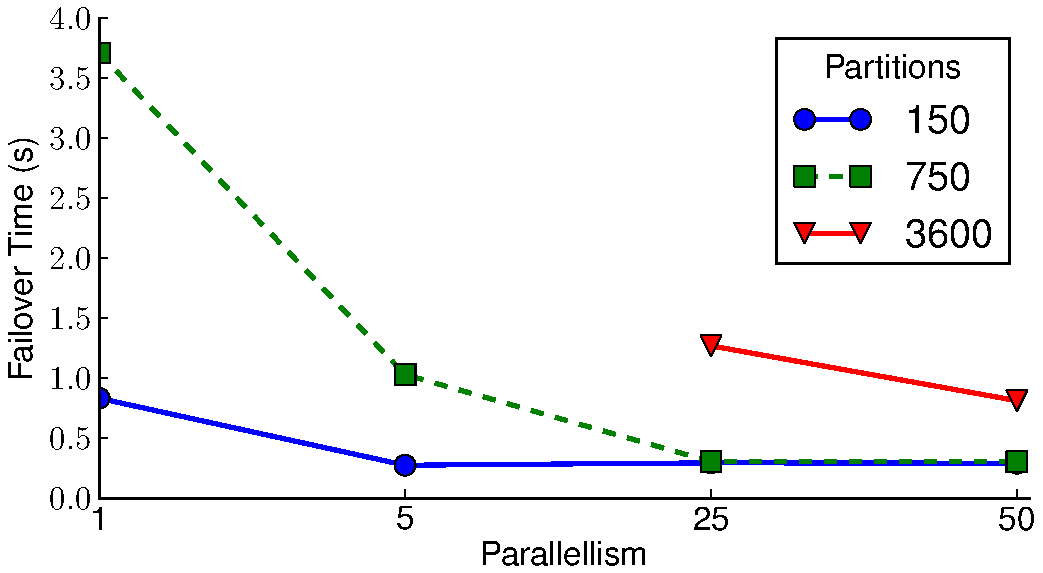
\includegraphics[width=0.90\textwidth]{failure.pdf}}
    \vspace*{-2ex}
    \caption{\label{fig:failure_detection} \ES transition parallelism vs. failover time.}
    \end{minipage}
    \vspace*{-2ex}
\end{figure*}


\eat{%%%%%%%
\begin{figure}[t]
    {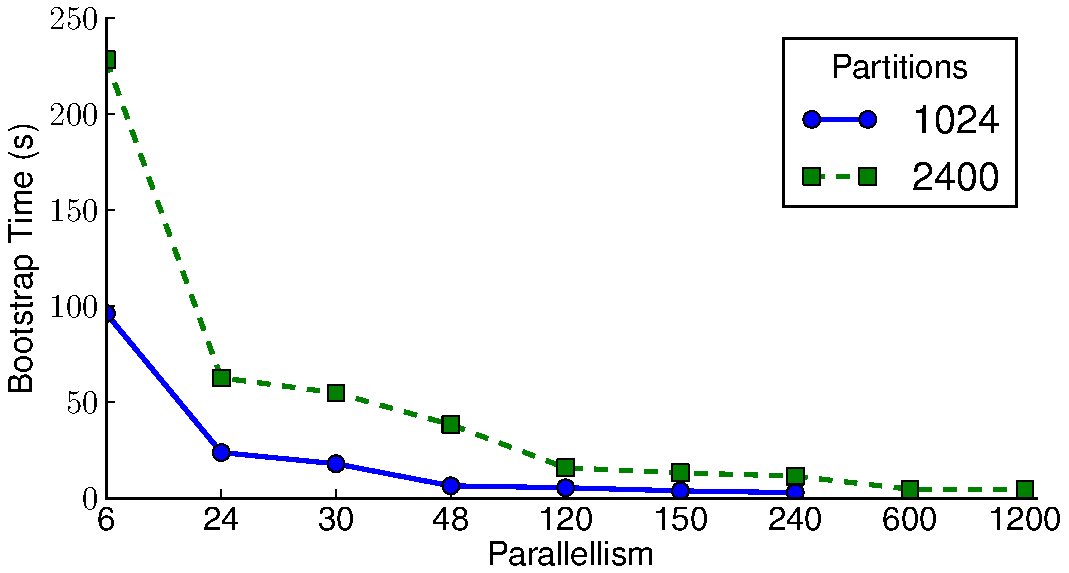
\includegraphics[width=\columnwidth]{bootstrap.pdf}}
    \vspace*{-2ex}
    \caption{\label{fig:bootstrap_time} \ES bootstrap time v/s parallelism.}
\end{figure}
}%%%%%%%%


Our first experiment examines \helix's performance when bootstrapping an \ES cluster,
(\ie adding the initial nodes and databases).  We note that while for some DDSs
bootstrapping is a rare operation, for others, like \databus consumers, it
happens frequently, and fast bootstrap times are crucial.

We vary the number of allowed parallel transitions, add nodes and an \ES
database, and then measure the time taken for the cluster to reach a stable
state.  We repeat the experiment for 1024 partition and 2400 partition
databases. 
Figure~\ref{fig:bootstrap_time} plots the result and shows that bootstrap time
decreases with greater transition parallelism, though the benefits diminish once
parallelism is in the tens of transitions.

The total bootstrap time is directly proportional to the number of transitions
required and inversely proportional to the allowed parallelism.  The number of
required transitions is a function of the number of partitions, number of
replicas per partition and the transitions drawn from \ES's state machine.
For example, an Espresso database with $p$ partitions and $r$ replicas requires
$pr$ offline$\rightarrow$slave transitions and $p$ slave$\rightarrow$master
transitions.  \ES sets allowed parallelism based on the number of cluster nodes
and the number of concurrent transitions a node can handle.
The final factor in deriving bootstrap time is the time required to execute each
individual transition.  These times are DDS dependent. 
For example, when an \ES partition enters the slave state \ES creates a \mysql
database and all required tables for it; this takes tens of milliseconds.
On bootstrap, this transition takes approximately 100 ms.  

\subsubsection{Failure Detection}
\label{sec:failuredetection}
%
One of \helix's key requirements is failure detection, and its performance in
this area must match what a DDS might achieve for itself with a custom solution.
In \ES, losing a node means all partitions mastered on that node become
unavailable for write, until \helix detects the failure and promotes slave
replicas on other nodes to become masters.
\eat{%%%%%%%
\begin{figure}[t]
    {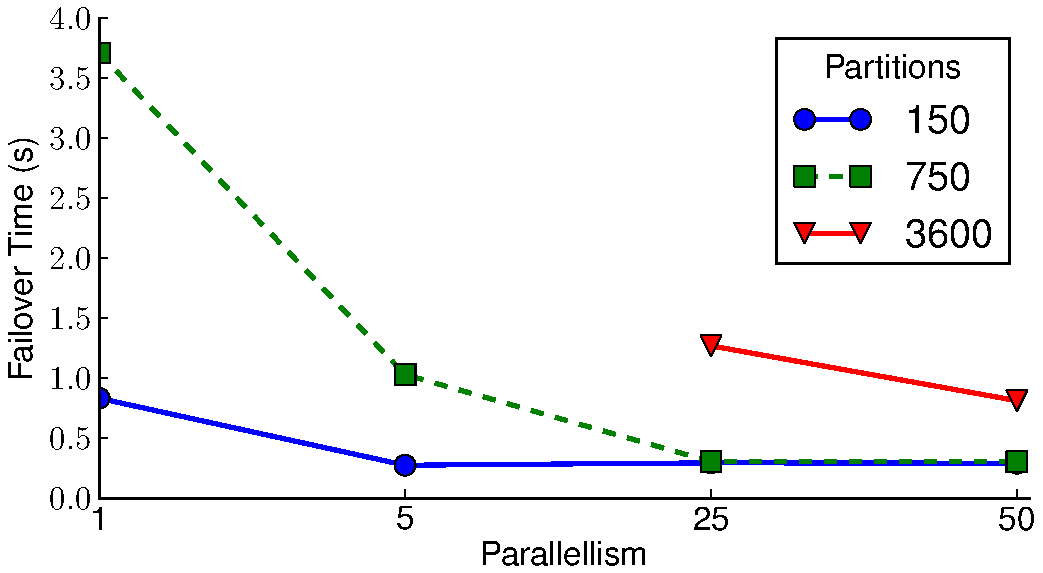
\includegraphics[width=\columnwidth]{failure.pdf}}
    \vspace*{-2ex}
    \caption{\label{fig:failure_detection} Failover time v/s parallelism}
\end{figure}
}%%%%%%%%%%
We run an experiment with an \ES cluster of size 6, randomly kill a single
node, and measure write unavailability.  We vary the the number
of \ES partitions and the maximum cluster-wide allowed parallel transitions.
Figure~\ref{fig:failure_detection} plots the result and shows most importantly
that we achieve low unavailability in the 100s of ms, and that this time decreases as we allow
for more parallel transitions.  It is interesting to note that earlier versions
of \helix had recovery times of multiple seconds.  The reason is that when so
many partitions transitioned from slave to master at once, \helix actually
bottlenecked trying to record these transitions in Zookeeper.  We ultimately
solved that bottleneck using techniques like group commit and asyncronous
reads/writes;  the key point is that we solved this problem for every DDS using \helix and masked
internal Zookeeper details from them.    

\subsubsection{Elastic Cluster Expansion}
\label{sec:elastic}
%
\begin{figure}[t]
    {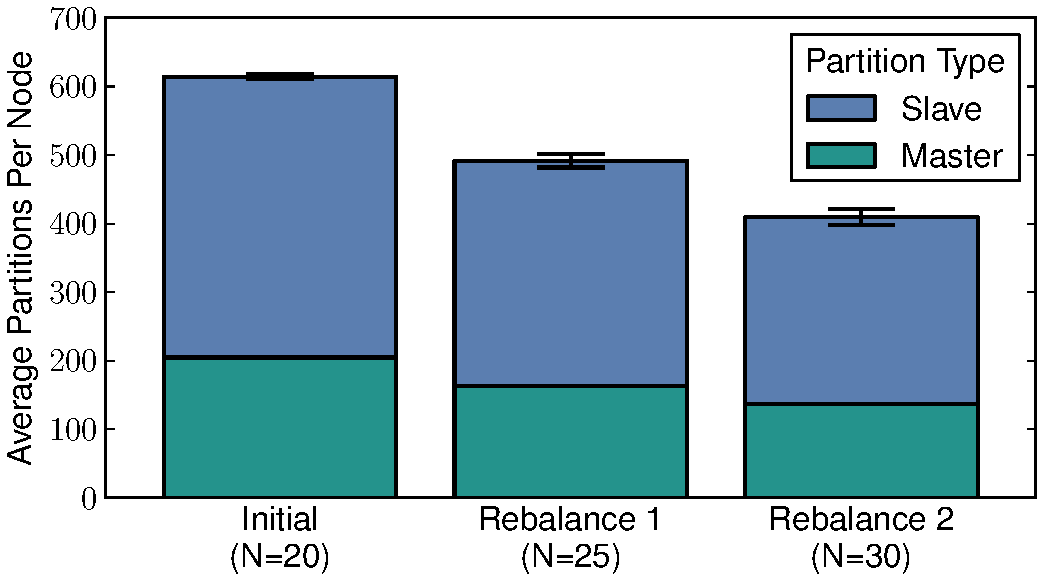
\includegraphics[width=\columnwidth]{rebalance.pdf}}
    \vspace*{-2ex}
    \caption{\label{fig:cluster_expansion} Elastic Cluster Expansion }
\end{figure}

Another of \helix's key requirements is its ability to incorporate new nodes as
clusters expand.  Recall Algorithm~\ref{alg:execution}
handles shifting partitions from existing to new nodes by computing target
states. 
We want to ensure rebalancing transitions as few replicas as possible; in
particular, in \ES, we want to ensure that the number of replicas transitioned to either
slave or master on new nodes is minimized, since these transitions typically
involve the expensive step of copying state.
We run an experiment that starts with a cluster with 20 nodes,
4096 partitions and 3 replicas per partition. We then add 5 new nodes, Helix
recalculates the placement and we find that 19.6\% of partitions are moved.  The
optimal percentage moved for full balance is clearly 20\%; with this
experiment's server and partition counts, achieving 20\% movement requires
moving partition fractions and so we instead achieve near balance.

Finally, we add an additional 5 nodes. After \helix recalculates the
placement we see that 16\% of partitions are moved, close to the optimal
solution. 
Figure~\ref{fig:cluster_expansion} shows we are minimal in
the number of partitions moved to ensure even load distribution.
While RUSH is very good at accomplishing this type of balancing, RUSH does not inherently support the 
concept of different replica states and is by default
designed for handling numbers of partitions that are orders of magnitude greater
than the number of nodes.  As discussed in Section~\ref{sec:design} we modified it to handle different states and
possibly much smaller numbers of partitions and still achieve close to minimal
movement.

\subsubsection{Planned Downtime}
\label{sec:downtime}
%
One function that \helix manages for DDSs is planned downtime, which helps for a
variety of administrative tasks, such as server upgrades.  In \ES bringing down
a node involves moving every partition on it to the offline state and
transitioning partitions on other servers to compensate. In fact, there
is a direct tradeoff between total time to complete planned downtime (\eg to
upgrade all nodes) versus accumulated unavailability over that time. 

Since Helix provides fault tolerance, a DDS system can upgrade its software by upgrading one node at a time. 
The goal of this exercise is to choose a reasonable tradeoff between minimizing
total upgrade time and minimizing unavailability during the upgrade. 
One simple approach is to upgrade one node at a time. 
Though this approach is common, it may leave a lot of parallelism on the table
that the DDS can handle and would speed up upgrade time.
Even though this is the most commonly used approach,
it is not guaranteed to achieve the two state goals.
The reason is if the ratio of transitions to max parallel transitions allowed on each node is very high, 
then its possible that overall availability of the system reduce.
The ideal solution is to have this ratio  close to 1. 

In this experiment we showcase the impact of concurrent partition migration on a
single node. We fix the total number of migrations at 1000 and control the
batch size of partitions that may be concurrently migrated. 

\begin{figure}[t]
    {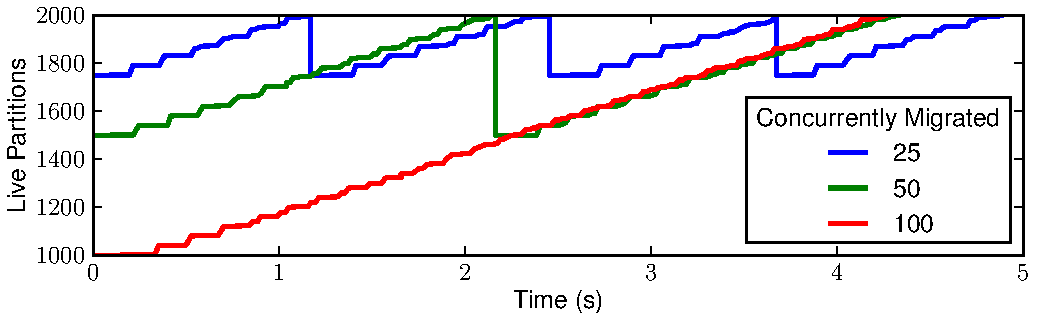
\includegraphics[width=\columnwidth]{migration-timeseries.pdf}}
    \vspace*{-2ex}
    \caption{\label{fig:migration_timeseries} Percentage of partitions that are
available over the course of a planned software upgrade.}
\end{figure}

\begin{figure}[t]
    {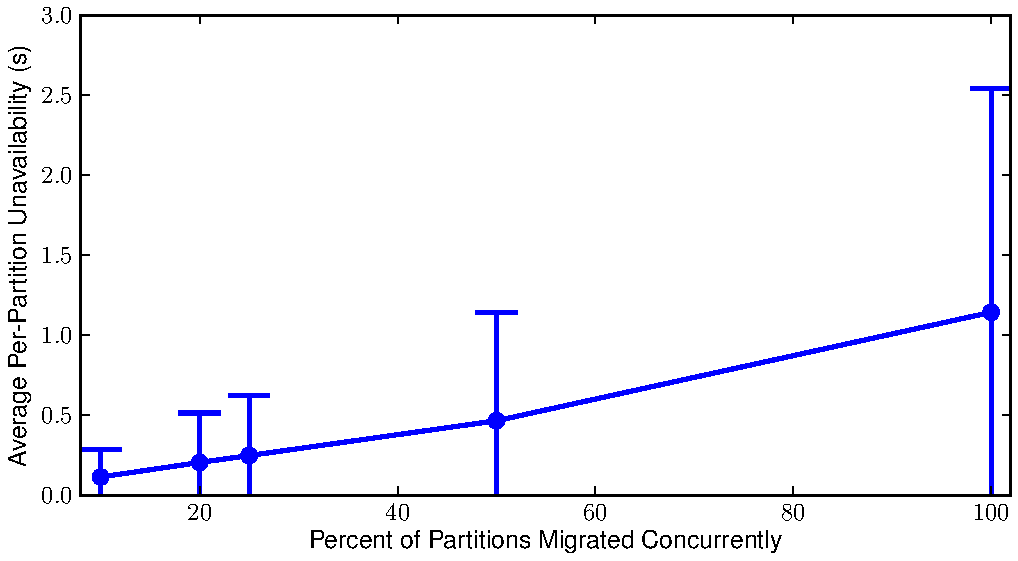
\includegraphics[width=\columnwidth]{average-migration.pdf}}
    \vspace*{-2ex}
    \caption{\label{fig:average_timeseries} Average unavailability per partition
during planned software upgrade.}
\end{figure} 

Figure~\ref{fig:migration_timeseries} shows that by choosing a lower concurrency
level, each migration is faster but the overall time taken to upgrade a node is larger.

Figure~\ref{fig:average_timeseries} shows a different perspective by plotting
the average per partition unavailability. It also shows that the variance grows
quite high as parallelism increases. While lower upgrade times are appealing,
higher error counts during upgrades are not.

The ability to balance downtime and unavailability is important for DDSs so the
upgrade process becomes smooth and predictable.  Beyond what is illustrated in
the scope of this experiment we also see cases where throttling transitions is
important to avoid load spikes that also affect availability.  For example,
bringing up too many \ES partitions online at the same time, when they have cold
caches, will cause failures.  By controlling transitions at the partition
granularity, \helix helps DDSs avoid availability and performance problems, and
manage planned downtime duration.

\begin{figure*}[t]
  \begin{minipage}[t]{0.48\textwidth}
    {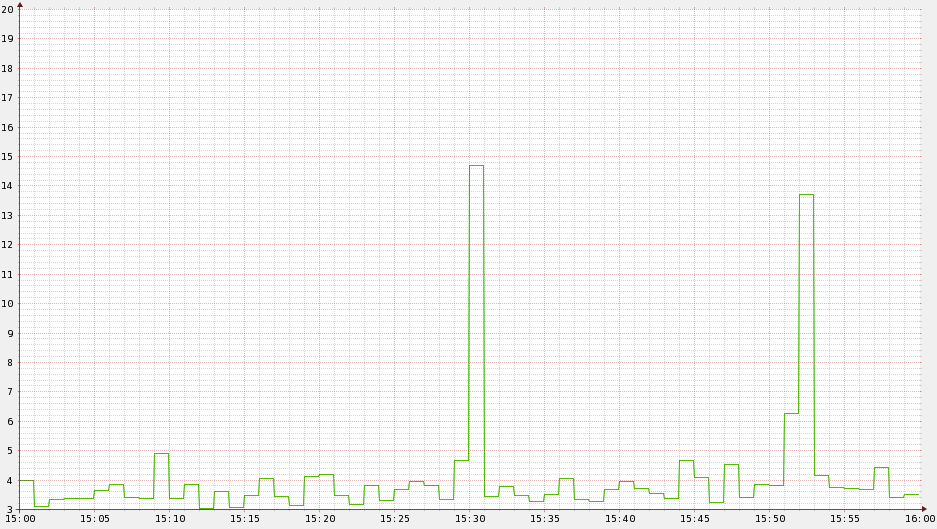
\includegraphics[width=0.99\textwidth]{expr/alert_graphs/latency99th_app74_alert_value.png}}
    \vspace*{-2ex}
    \caption{\label{fig:latency_alert} Alert reporting 99th percentile latency
on a single \ES node.}
  \end{minipage}
  \hfill
  \begin{minipage}[t]{0.48\textwidth}
    {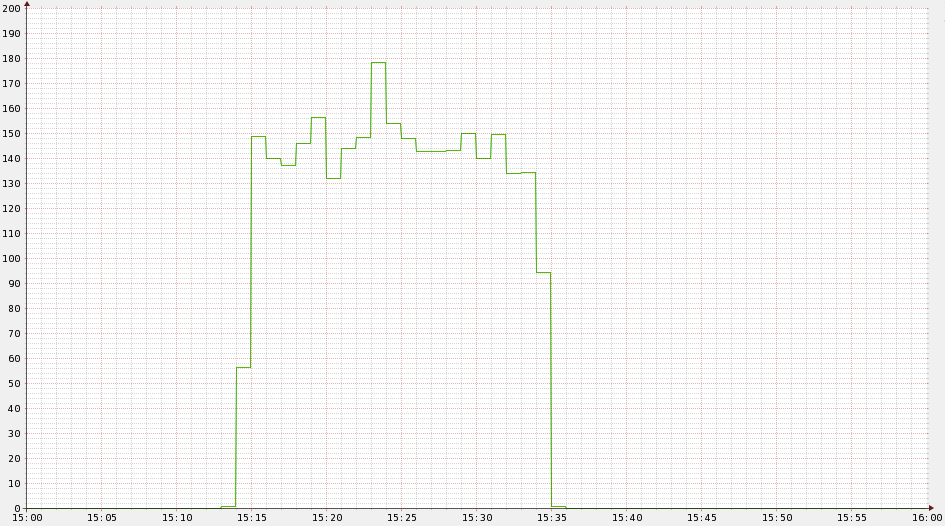
\includegraphics[width=0.99\textwidth]{expr/alert_graphs/errorcount_sumeach_alert_val.png}}
    \vspace*{-2ex}
    \caption{\label{fig:error_alert} Alert reporting the cluster-wide \ES error count.}
    \end{minipage}
    \vspace*{-2ex}
\end{figure*}

\subsubsection{Alerts}
%
Recall from Section~\ref{sec:design} that \helix provides DDSs a framework for
defining monitored statistics and alerts.  Here we give some examples of alerts
\ES runs in production.

\ES monitors request latency to ensure it is meeting its SLAs or take
corrective action otherwise.  Specifically it registers the alert \\
\texttt{decay(1)(node*.latency99th) > 100ms}  \\
Since the alert is wildcarded on node name, we separately monitor 99th
percentile latency on each node in the \ES cluster.  The decaying sum setting of 1
means we monitor the latest reported value from each node, and ignore older
values.  Figure~\ref{fig:latency_alert} shows a production graph displaying the current monitored value for a
particular \ES node.  The x and y axes are wall time and requiest latency,
respectively.  A similar graph (not shown here) indicates whether the
alert is actually firing and, when fired, emails notification to \ES operators.

A second alert monitors the cluster-wide wide request error count: \\
\texttt{decay(1)(node*.errorcount)|SUMEACH > 50ms}  \\
The alert is again wildcarded on node name, but now computes the sum of errors
over all nodes.  Figure~\ref{fig:error_alert} shows the production graph and,
again, there is an unshown corresponding graph displaying the alert status.

%Template for displaying graphs
\eat{%%%%%%%%%%
\begin{figure*}[t]
  \begin{minipage}[t]{0.48\textwidth}
    {\includegraphics[width=0.85\textwidth]{experiments/load/load1K.eps}}
    \vspace*{-2ex}
    \caption{\label{fig:load1K} Load times for 120 million 1K records.}
  \end{minipage}
  \hfill
  \begin{minipage}[t]{0.48\textwidth}
    {\includegraphics[width=0.85\textwidth]{experiments/load/vary_rec_size.eps}}
    \vspace*{-2ex}
    \caption{\label{fig:vary-rec-size} Load times for 120GB, varied record
size.}
    \end{minipage}
    \vspace*{-2ex}
\end{figure*}
}%%%%%%%%%

\section{Related Work}
\label{sec:related}
%
The problems that systems dealing with cluster management attempt to solve fall in 3 main categories:
(a) resource management, (b) enforcing correct system behavior in the presence
of faults and other changes, and (c) monitoring. 

There are generic systems that solve resource management and monitoring, but not
fault-tolerance, in a generic manner.  Other DDSs support fault-tolerance and
enforce system behavior correctness in a way that is specific to that particular
DDS.

\subsection{Generic Cluster Management Systems}

Systems such as YARN~\cite{yarn} and Mesos~\cite{mesos} implement resource management and 
some monitoring capabilities in a generic way. Applications using these systems are responsible 
for implementing the specific logic to react to changes in the cluster and enforce correct system behavior. 
We detail Mesos an example.

Mesos has 3 components: \emph{slave daemons} that run on each cluster node, a
\emph{master daemon} that manages the slave daemons, and \emph{applications} that 
run tasks on the slaves.
The master daemon is responsible for allocating resources (cpu, ram, disk) across
the different applications. It also provides a pluggable policy to allow for
adding of new allocation modules.
An application running on Mesos consists of a \emph{scheduler} and an
\emph{executor}.  The scheduler registers with the master daemon to request
resources. The executor process
runs on the slave nodes to run the application tasks. The master daemon determines how many
resources to offer to each application. The application scheduler is responsible
for deciding which offered resources to use.  Mesos then launches the tasks on
the corresponding slaves.
Unlike Helix, Mesos does not provide a declarative way for applications to
define their behavior and constraints on it and have it enforced automatically,
but provides resource allocation functionality that is complementary to Helix.

\subsection{Custom Cluster Management}

As mentioned before, distributed systems like PNUTS~\cite{cooper08},
Hbase~\cite{hbase}, HDFS~\cite{hadoop}, and MongoDB~\cite{mongodb} implement 
cluster management in those specific systems. As an example, we examine
MongoDB's cluster management. 

MongoDB provides the concept of document collections which are sharded into
multiple chunks and assigned to servers in a cluster. MongoDB uses range
partitioning and splits chunks when chunks grow too large. When the load of any
node gets too large, the cluster must be rebalanced by adding more nodes to the
cluster and some chunks move to the new nodes.

Like any other distributed system, MongoDB must provide failover capability and
ensure that a logical shard is always online. To do this, MongoDB assigns n
servers (typically 2-3) to a shard. These servers are part of a replica set.
Replica sets are a form of asynchronous master-slave replication and consist of
a primary node and slave nodes that replicate from the primary. When the primary
fails, one of the slaves is elected as the primary.  This approach to fault
tolerance is similar to the MasterSlave state model \ES uses; \ES gets it for
free from \helix, while MongoDB had to build it.

Other distributed systems implement very similar cluster management
capabilities, but each system reimplements it for itself, and not in a way that
can be easily reused by other systems. 

\subsection{Domain Specific Distributed Systems}

Hadoop/MapReduce~\cite{hadoop,dean04} provides a programming model and
system for 
processing large data sets. It has been wildly successful, largely because it
lets programmers focus on their jobs' logic, while masking the details of the
distributed setting on which their jobs run.  Each MR job consists of multiple map and reduce jobs 
and the processing slots get assigned to these jobs. Hadoop takes care of monitoring 
the tasks and restarting tasks in case of failures.  Hadoop, then, very
successfully solves the problems we outline for cluster management, but only in
the MR context.  \helix aims to bring this ease of programming to DDS
development.

Zookeeper~\cite{zookeeper} is a centralized service for maintaining configuration information, 
naming, providing distributed synchronization, and providing group services. 
It is used by many distributed systems to help implement cluster management
functionality, and we of course use it heavily as a building block in \helix.  It is important to
note that Zookeeper alone does not solve the cluster management problems.  For
example, it provides functionality to notify a cluster manager when a node has
died, but does not plan and execute a response. 

\subsection{Distributed resource management}
%
A number of older systems pioneered solutions in distributed resource
management.  Amoeba~\cite{tanenbaum90}, Globus~\cite{frey02}, GLUnix~\cite{ghormley98} and 
Legion~\cite{chapin99} all manage large numbers of
servers and present them as a single, shared resource to users.  The challenges
they tackle most relevant to \helix include placing resources, scheduling jobs, monitoring 
jobs for failures, and reliably disseminating messages among nodes.  Much of the
scheduling work relates closely to how we distribute resource partitions among
nodes, and how we hope to make this distribution more dynamic in the future,
where \helix will move partitions aggressively in response to load imbalance.
On the other hand, we address failure monitoring in \helix with Zookeeper,
which itself relates closely to these systems.  In general, it is easy to see
the lineage of these systems reflected in \helix.

\section{Conclusion}
\label{sec:conclusion}
%
At \linkedin we have built a sophisticated infrastructure stack of DDSs, including
offline data storage, data transport, data serving and search systems.  This
experience has put us in great position to observe the complex, but common,
cluster management tasks that pervade all of our DDSs.  This motivated us to
build \helix.  We designed \helix with a diverse set of DDSs in mind to ensure
its generality.

\helix lets DDSs declare their behavior through a set of pluggable interfaces.
Chief among these interfaces are a state machine that lets the DDS declare the
possible states of their partitions and transitions between them, and constraints 
that must met for each partition.  In this way, DDS designers concentrate on
the logic of the system, while the \helix execution algorithm carries out transitions in the distributed
setting.  

We have had a lot of success with \helix at \linkedin.  By providing the
performance and functionality a DDS would normally target for itself, we have indeed
offloaded cluster manager work from a number of DDSs.  \helix even lets these DDSs
make what would normally be drastic changes to the way they are managed with
just minor changes to the \helix state model.    

We have a number of future directions for \helix.  One of them is to simply
increase its adoption, a goal we expect our open-source release to accelerate.
A second goal is to manage more complex types of clusters.  The first challenge
is to handle heterogenous node types; we plan to approach this with the notion
of \emph{node groups}.  We cluster nodes by capabilities (cpu, disk capacity,
\etc) and weight more performant groups to host larger numbers of partitions. 
The second challenge is to manage clusters over increasingly complex network
topologies, including those that span multiple data centers.  

A third goal is to push more load balancing responsibility into \helix.  \helix's
alerting framework lets it observe imbalance, and we must continue to extend the
\helix execution algorithm to to respond to imbalance, yet remain completely
generic across DDSs. 

\section{Acknowledgements}
\label{sec:Acknowledgements}


In addition to the Helix team, many other members of the Linkedin Data Infrastructure team helped significantly in the development of Helix. 
The initial work on Helix came out of the Espresso project. The Espresso team and in particular, Shirshanka Das
, Lin Qiao, Swaroop Jagadish and Aditya Auradkar worked closely with us driving
the requirements and shaping some of the ideas. Chavdar Botev, Phanindra Ganti and Boris Shkolnik
from the Databus team and Rahul Aggarwal, Alejandro Perez, Diego Buthay, Lawrence Tim, Santiago from the Search team were 
early adopters and helped solidify the early versions. David Zhang, Cuong Tran, Wai Ip were instrumental in stress
testing Helix and improving the quality and performance.
%\section{Miscellaneous}
Here is stuff that may be needed later.


{\em Take an example here to map the terms.  Most distributed systems
at a high level can be tasks, partitions/replicas and its state. In
this paper, we use these terminolgies to explain Helix design and
implementation. Its important to note that these are fairly generic
terms and can be mapped to different things based on the system. For
example, in a data serving system each task can be a database and if
the database is sharded, each partition is a shard. Similarly in a pub
sub system, a task can be a Topic/Queue and in a search system it can
refer to an Index.  }

%------------------------------------------------
Helix needed a way to map partitions to nodes.
tasks, partition/replica and its state.
Given that partitions are distributed among various nodes in the
cluster for performance, scalability and operability, the first {\em
  thing} that Helix needed was a various partition assignment algorithms. 
One of the commonly used
algorithm is consistent hashing. The most important goal on any
assignment is distribute the partitions evenly(assuming they are equal
weight) among all the nodes in the cluster.




In this section we will cover how the state
machine with constraints is
satisfied in Helix in a generic way. As we see
in our previous section one would
simply provide the following for each resource
in the system
* Number of partitions
* Number of Replicas for each partition
* State Machine with valid states and state
* transitions
* Constraints on state and state transition.

{\em 
Justify any interesting design decisions, and the theme is to
emphasize how they help Helix be generic.

Think about giving anecdote about how we easily spun Espresso w/mysql
replication from Espresso w/databus replication.  Repeat this in
evalation.

Limitations/negatives
\bi
\item What are the possible problems?
\item Why aren't we worried about them right now?
\item What are possible solutions if we want to address them.
\ei


Note about ideal state terminology.
\bi
\item 
We want to describe the set of constraints and
optimization goals as 1 thing, and an actual
config that achieves those goals as a 2nd
thing.
\item The first thing can be described as an
optimization problem: maybe "optimization
spec?"
\item The second thing is a solution: maybe
``assignment''
\ei


Consider merged impl with this section if it makes sense


Even though all distributed systems share the common terminologies,
they differ from each other in the way partitions are distributed
among nodes, states associated with each replica of the partition.
}

\section{Formalisms}

This section formalizes the description of a DDS, informally introduced
in Section~\ref{Informal}.

\begin{definition}
Let \(R = \{r_1, r_2, \ldots r_{N_R}\}\) be a set of resources. 
\end{definition}

\begin{definition}
Let the number of resources be \(N_R\)
\end{definition}

\begin{definition}
Each resource \(r \in R\) has a set of partitions
\(P(r) = \{p^r_1, p^r_2, \ldots p^r_{N_(r)}\}\).
\end{definition}

\begin{definition}
Let \(N(r)\) be the number of partitions for resource \(r \in R\). 
\end{definition}

\begin{definition}
Let \(M = \{m_1, m_2, \ldots m_{N_I}\}\) be a set of machines or 
or nodes or instances.  
\end{definition}

\begin{definition}
Let \(N_M\) be the number of machines.
\end{definition}

We group the nodes into a mutually exclusive and exhaustive set of zones.

\begin{definition}
Let \(Z = \{z_1, z_2, \ldots z_{N_Z}\}\) be a set of  zones such that 
(i) \(z_i \subseteq M\) 
(ii) \(\forall i \forall j , i \neq j \Rightarrow z_i \cap z_j = \phi \) 
(iii) \(\cup_i z_i = M\)
\end{definition}

\begin{definition}
Let \(N_Z\) be the number of zones.
\end{definition}

Since resources use machines in common, there is clearly interplay
between actions performed on different resources. Nonetheless, at this
point in the discussion, we consider resources independently. 
We focus on a single resource and write the set of \(N_P\) partitions 
as \(P = \{p_1, p_2, \ldots p_{N_P}\}\). 

\begin{definition}
\label{defn_states}
Let \(S\) be a set of states.  
\end{definition}

We define the state of the system when it is quiescent as follows.

\begin{definition}
\label{defn_q1_system_state}
The {\bf state} \(U\) of a system at a given point in time
is defined as a set of tuples, 
\(\{(p, s, m)\} \).  A tuple \((p, s, m)\) tells us that
partition \(p \in P\) exists in state \(s \in S\) on machine \(m \in M\). 
\end{definition}

%-----------------------------------------------------
We {\em must} define which state transitions are legal 
--- Definition~\ref{defn_legal_transition}.
\begin{definition}
\label{defn_legal_transition}.
Let \(S_L \subseteq S^2 =  S \times S\) be a set of
legal state transitions. For example, \((s_i, s_j) \in S_L
\Rightarrow\) it is legal for a partition to transition from state 
\(s_i\) to state \(s_j\).
\end{definition}
%-----------------------------------------------------
We {\em may} define a partial ordering on the state transitions.
\begin{definition}
\label{defn_state_trans_partial_order}
Let \(S_P \subseteq S_L \times S_L\) be a set of state transitions such
that \(((s_1, s_2), (s_3, s_4)) \in S_P\) indicates that the transition
\((s_1, s_2)\) should be executed in preference to the transition
\((s_3, s_3)\).
\end{definition}
%-----------------------------------------------------

We {\it may} impose requirements for each \(s
\in S\) as in Invariant~\ref{inv_state_count_bound1}
\begin{definition}
Let \(Count(p', s') = |\{(p, s, m) | (p, s, m) \in U \wedge p = p' \wedge s =
s'\}|\) be the number of machines in which partition \(p'\) is in state
\(s'\)
\end{definition}


\begin{invariant}
\label{inv_state_count_bound1}
\(R_X(s) = (lb, ub) \Rightarrow \forall p, lb \leq Count(s, p) \leq ub
\) says that the number of machines in state \(s\) is {\bf expected} to
be between \(lb\) and \(ub\) on all partitions.
\end{invariant}

\begin{invariant}
\label{inv_one_state_for_one_partition_on_one_machine}
Note that a partition cannot be in 2 different states on the same
machine i.e., \((p_1, m_1, s_1) \in U \Rightarrow (p_1, m_1, s_2) \not
\in U\).
\end{invariant}

Since the behavior of
one partition can be reasoned about independent of the state of other
partitions, it simplifies notation to assume that there is only one
partition. We can 
re-write Definition~\ref{defn_q1_system_state} as 
Definition~\ref{defn_q_system_state}, 

\begin{definition}
\label{defn_q_system_state}
The {\bf state} \(U\) of a system at a given point in time
is defined as a set of tuples, 
\(\{(m, s)\} \).  A tuple \((m, s)\) tells us that
machine \(m \in M\).  is in state \(s \in S\) on 
\end{definition}

When Helix is running, there are external events that cause the state of
the system to be undesirable. For example, a machine may go down or
become over-loaded, another machine may come on-line or may become
lightly loaded. It is the job of Helix to respond to external stimuli by
changing the state of the system. In doing so, it is important to
remember what Brutus\footnote{Julius Caesar, Act II, Scene i},  
eloquently stated as 
\begin{verse}
{\em 
Between the acting of a dreadful thing \\
And the first motion, all the interim is \\ 
Like a phantasma or a hideous dream; \\
}
\end{verse}

What does this mean in our context? It means that when one issues a
directive to a machine to change state, there is an unpredictable amount
of time that elapses between the issuance of the directive and the
notification of it having taken effect. The kind of change we can
request is in Definition~\ref{defn_change}.

\begin{definition}
\label{defn_change}
A change is a tuple of the form \((m, s_1, s_2)\) indicating a (legal) request to
change machine \(m\) from state \(s_1\) to state \(s_2\). Note that
\(s_1 \neq s_2\) and and \((s_1, s_2) \in S_L\)
\end{definition}

\begin{definition}
\label{defn_apply_change}.
The application of a change \((m, s_1, s_2)\) to a quiescent state \(U\) 
results (at some future point in time) in a new state \(U'\) such that 
\((m, s_2) \in U'\), assuming that \( (m, s_1) \in U\).
\end{definition}

\begin{definition}
\label{defn_system_change}
Let the ``change set'' \(U_D\) be the set of change requests (Definition~\ref{defn_change}). 
that have been issued but have not yet been processed. We can also view
this as the dynamic analog of Definition~\ref{defn_q_system_state}. Note
that there can be {\bf only one} change request for a given machine 
\end{definition}

Given that there is uncertainty in the state of a machine, we
re-write Invariant~\ref{inv_state_count_bound1} as 
Definition~\ref{defn_d_state_count}.

\begin{definition}
\label{defn_d_state_count}
\(R_D(s) = (s, lb, ub) \Rightarrow lb \leq Count(s) \leq ub
\) says that the number of machines in state \(s\) in a {\bf D}ynamic
system {\bf is} between \(lb\) and \(ub\).
\end{definition}

The overall state count is \(R(D)\), defined in
Definition~\ref{defn_d_state_count_overall}
\begin{definition}
\label{defn_d_state_count_overall}
\(R_D = \{R_D(s)\}\)
\end{definition}

So, we model the flux that Helix must contend with as a dance between 
\bi
\item Helix issuing change requests (Definition~\ref{defn_change}) that get
added to \(U_D\) (Definition~\ref{defn_system_change}). This 
increases the uncertainty in our knowledge of the system. 
In terms of our notations, the
difference between \(lb\) and \(ub\) for some \((s, lb, ub) \in R_D\)
increases.
\item the system responding with notifications that decreases the
uncertainty.
In terms of our notations, the
difference between \(lb\) and \(ub\) for some \((s, lb, ub) \in R_D\)
decreases.
\ei

We can model this as a producer/consumer relationship where Helix is the
producer and the system is the consumer and the result of a change is
defined in Definition~\ref{defn_apply_change}. Consider a change request
of the form \((m, s_1, s_2)\) 
\bd
\item [PRODUCER] Change request is made
\be
\item \((m, s_1, s_2)\) is added to \(U_D\). 
\item Change to \(R_D\) is as follows
\bd
\item [PRIOR] \((s_1, l_1, u_1), (s_2, l_2, u_2) \in R_D\) 
\item [POSTERIOR] \((s_1, l_1-1, u_1), (s_2, l_2, u_2+1) \in R_D\)
\ed
\ee
\item [CONSUMER] Change request is satisifed
\be
\item \((m, s_1, s_2)\) is deleted from \(U_D\) and 
\bd
\item [PRIOR] \((s_1, l_1-1, u_1), (s_2, l_2, u_2+1) \in R_D\)
\item [POSTERIOR] \((s_1, l_1-1, u_1-1), (s_2, l_2+1, u_2+1) \in R_D\)
\ed
\ee
\ed

\subsection{Executing a change set}

\subsubsection{Motivation}
We have decribed what happens when a single change is applied. Assume
that we had a set of changes to apply. 
We would like to execute as many of these changes in parallel. However,
when we execute them in parallel, we have no guarantee on the order in
which they will execute. Which means that unless we are confident that
{\em all} execution orders are valid, we should {\em not} run them in
parallel.  

The user {\it may} also impose an ordering on state transitions. In
other words, if have a choice between executing change \((m_1, s_{11},
s_{12})\) and \((m_2, s_{21}, s_{22})\), then we execute the
change with the higher priority --- Definition~\ref{defn_priority}

\begin{definition}
\label{defn_priority}
There exists a many-to-one mapping from \(P: S_L \rightarrow I^+\) such
that \\
\(((s_{11}, s_{12}), p_1), (s_{21}, s_{22}), p_2)) \in P
\wedge p_1 < p_2 \Rightarrow (s_{11}, s_{12}) \) has higher priority
than \((s_{21}, s_{22}) \) 
\end{definition}

We are now in a position to state the problem of executing a change set
in parallel.
\begin{definition}
\label{defn_the_problem}
Given the state of the system, in terms of \(R_D\) and \(U_D\) and 
a change set, find the largest subset of it which respects
Definition~\ref{defn_priority} and
Invariant~\ref{inv_state_count_bound1}.
\end{definition}

%% On a more pragmatic note, we must bear in mind that we are working
%% against a dynamic system where machines can go down and come back up in
%% unpredictable ways. So, there is little point in spending a lot of time
%% planning a perfect execution plan and then having it come to naught
%% because of external factors.
%% This was stated more eloquently as \footnote{work of devotion
%% written in Latin by Thomas Kempis.}
%% \begin{center}
%% {\em 
%% Man proposes but God disposes
%% }
%% \end{center}

\begin{definition}
A row \((s_1, s_2, n, r)\) of Table~\ref{State_Transition_Count}
indicates that there are \(n\) machines in \(U_D\) that need to
transition from state \(s_1\) to \(s_2\)
\end{definition}

Figure~\ref{algo} presents the algorithm for Definition~\ref{defn_the_problem}.

\begin{figure}
\centering
\fbox{
\begin{minipage}{8 cm}
\centering
\begin{tabbing} \hspace*{0.25in} \= \hspace*{0.25in} \= \kill
1. \> Create Data Structure in Table~\ref{State_Transition_Count}, sorted
descending on priority \\
\> Process the table a row at a time. Let \(m'\) be the number of
machines \\ 
2. \> For each row, find the largest value of \(m \leq m'\) such that \\
\> \(m\) can be applied without violation of any constraint
\end{tabbing}
\end{minipage}
}
\label{algo}
\caption{Algorithm A for Definition~\ref{defn_the_problem}}
\end{figure}

\begin{table}
\centering
\begin{tabular}{|l|l|l|l|} \hline \hline
{\bf From State} & {\bf To State} & {\bf Number of} & {\bf Priority} \\ 
                 &                & {\bf Machines} &                \\ \hline \hline
\(s_1\) & \(s_2\) & 3 & 1 \\ \hline 
\(s_2\) & \(s_3\) & 4 & 2 \\ \hline 
\(s_1\) & \(s_3\) & 1 & 2 \\ \hline 
--- & --- & --- & --- \\ \hline 
\hline
\end{tabular}
\caption{Sample of Count of Transitions to be made}
\label{State_Transition_Count}
\end{table}
%------------------------------------------------------
\begin{theorem}
The complexity of algorithm A is \(O(M_P)\). This follows from the fact 
that the maximum number of state transitions that can occur for that
partition.
\end{theorem}

\begin{proof}
\TBC
\end{proof}

\section{Modeling Usage Examples in Helix}

\subsection{\GP\ in Helix}
\label{Galapagos_in_Helix}
When deployed as part of \GP (Section~\ref{Galapagos}), Helix is
configured as 
\be
\item \(S = \{M, S, O\}\), where \(M =\) Master, \(S =\) Slave, \(O =\)
Offline (Definition~\ref{defn_states}) {\bf TO BE CORRECTED}
\item When a node comes online, it generates significant network
traffic. Throttling network traffic is modeled as \(R_D(S) = (S, lb, ub)
\Rightarrow ub - lb \leq 3\) (Definition~\ref{defn_d_state_count})
\item \TBC
\ee

\subsection{YARN in Helix}
\label{YARN_in_Helix}

Describe how Helix {\it could} have been used by YARN \TBCKG
%------------------------------------------------
\section{Operational Ease}
\label{Operational_Ease}

Having defined how our system {\it should} operate, we would like to
know how the system {\it does} operate.  For example,
Section~\ref{Espresso_in_Helix} indicates that there should be exactly
one master for each partition. From an Ops perspetive though (knowing
that nodes fail), it is more important to know {\em how often} this
was violated than {\em whether} it was violated.

In general, we would like to know the fraction (percentage) of time
during which there were \(n\) instances in state \(S_1\) for \(n =
0,1, \ldots\). Since this is different for different partitions, we
sum the times across the partitions.
Table~\ref{tbl_master_time_stats} shows us that the percentage of time
when a partition had no master was 2.69\%. Whether this is acceptable
or not depends on the SLA that the Ops team has established with the
business owner. What is important to note is that
\be
\item This kind of log analysis comes ``out-of-the-box'' with Helix
\item Helix makes it easy to have such a structured discussion.
\ee
\begin{table}[h]
\centering
\begin{tabular}{|l|l|} \hline \hline
{\bf Number of Instances} & {\bf Time (in sec) } \\ \hline \hline
0 & 20384093 \\ \hline 
1 & 734689509 \\ \hline 
\hline 
\end{tabular}
\caption{Time Statistics for state MASTER}
\label{tbl_master_time_stats}
\end{table}

% \subsection{Time Statistics for State Slave in \ES}
% \label{time_stats_for_slave}
% See Table~\ref{tbl_slave_time_stats}
% \begin{table}[h]
% \centering
% \begin{tabular}{|l|l|} \hline \hline
% {\bf Number of Instances} & {\bf Time (in sec) } \\ \hline \hline
% 0 & 9586805 \\ \hline 
% 1 & 23092725 \\ \hline 
% 2 & 721804536 \\ \hline 
% 3 & 589536 \\ \hline 
% \hline 
% \end{tabular}
% \caption{Time Statistics for state SLAVE}
% \label{tbl_slave_time_stats}
% \end{table}

%



\vspace{5ex}

{\small
\bibliographystyle{abbrv}
\bibliography{helix}
}


\end{document}
